\documentclass[11pt,a4paper,twocolumn]{article}

% --- packages ---
\usepackage[T1]{fontenc}
\usepackage[utf8]{inputenc}
\usepackage{lmodern}
\usepackage[margin=2cm,columnsep=0.7cm]{geometry}
\usepackage{microtype}
\usepackage{tikz}
\usetikzlibrary{positioning,arrows.meta,shapes.geometric,decorations.pathreplacing,calc,fit,backgrounds,matrix,shapes.misc}
\usepackage{booktabs}
\usepackage{caption}
\captionsetup{font=small,labelfont=bf}
\usepackage[round,authoryear]{natbib}
\usepackage{xcolor}
\usepackage{enumitem}
\setlist{nosep,leftmargin=*}
\usepackage{hyperref}
\hypersetup{colorlinks=true,linkcolor=black,citecolor=black!60!blue,urlcolor=blue!60!black}

% --- title ---
\title{\textbf{Shared Substrate}\\[2pt]
{\large A Discipline for Sustained Human--AI Coupling on Complex Problems}}
\author{Oleg Roshka}
\date{August 2026 --- draft v0.2\\[3pt]
{\small Paper source and companion materials:
\url{https://github.com/olegroshka/shared-substrate}}}

\begin{document}
\twocolumn[
\begin{@twocolumnfalse}
\maketitle
\begin{abstract}
\noindent
Modern AI agents have characteristic limitations on long-horizon
complex work: bounded context windows, drift across iterations,
phantom decisions (claims of resolution not grounded in any
artefact), reference rot, lost intent, and the cost of restarting
cold each session. These limits will not be dissolved by larger
models --- they are limits of \emph{substrate}, the externalised
state any sustained reasoning must traverse. We articulate
\textbf{Shared Substrate}: a discipline the author has practised
across many domains and many years of sustained complex work, made
explicit here in response to the demands of multi-session AI
collaboration --- the discipline of forming, maintaining, and
cascading hierarchical external representations across the
manifestation trajectory of a project. The organising image is the
\emph{centroid}: the participants in sustained work --- the human
operator, AI agents, successive model generations, colleagues ---
are noisy point masses in motion, and the substrate is the
deliberately \emph{pinned} centre of mass of that ensemble.
Session drift is excursion; warm-up is reversion; the discipline
is what holds the centroid stationary. The discipline rests on
long-standing cognitive-science foundations --- distributed
cognition \citep{hutchins1995}, external representations
\citep{scaife1996external}, cognitive load
\citep{sweller1988cognitive}, hierarchical levels of analysis
\citep{marr1982vision}, boundary objects \citep{star1989boundary}
--- recovers software-engineering precedent (Architectural
Decision Records \citep{nygard2011adr}, Single Source of Truth,
hexagonal architecture \citep{cockburn2005hexagonal}, append-only
logs \citep{candea2003crashonly}) alongside emerging agentic-AI
patterns \citep{lewis2020rag, packer2024memgpt, shinn2023reflexion,
bai2022constitutional}, and is grounded formally: each abstraction
layer of a project is paired with a representation formalism and a
verification oracle --- from executable behavioural contracts at
the topmost layer to measurable non-functional envelopes at the
operational one --- with the work's state kept observable to the
agents themselves, closing the feedback loop that enforces
guardrails while divergence is still cheap to correct. The
substrate that results is best understood as a compressed
representation of the thing being manifested --- agentic
pipelines expand it into the work, and the human deposits only
what no pipeline can derive --- so the discipline's purpose has a
one-line statement: separate genuine human creative input from
cognitive load. The discipline defines six artefact categories
--- Knowledge Bases, Inventories, Data Dictionaries, Decision
Records, Open Questions, Glossary --- a status lifecycle, an edit
protocol with explicit anti-patterns and a trivial-fix lane, and
forward/reverse propagation rules across the hierarchy. Its
posture is \emph{human-governed, agent-executed}: a five-layer
adoption stack progressively delegates substrate execution to
agents while intent, decision, and scope authority remain with the
person. The practice is domain-agnostic --- software engineering
appears here only as the worked instance --- and practicable today
with no special tooling. We claim the substrate matters as much as
the model, and that this is the form of work AI raises in
importance --- not invents.
\vspace{6pt}
\end{abstract}
\end{@twocolumnfalse}
]

% =====================================================================
\section{Why Substrate Matters as Much as Model}
% =====================================================================

Most discussions of AI capability concern the model: its parameters,
its benchmarks, the length of its context window. Almost none concern
the \emph{substrate} --- the externalised state any sustained
reasoning, whether organic or artificial, must traverse. This paper
is about the substrate.

The thesis is simple to state and difficult to live up to.
\textbf{For complex tasks that span many sessions, many decisions,
and many abstraction layers, the substrate matters at least as much
as the model.} A larger model with no substrate degrades along
predictable axes; a moderate model with a well-tended substrate can
sustain coherence over arbitrary horizons. Bigger context windows
are a quantitative response to a qualitative problem. They postpone
the failure modes; they do not dissolve them.

By \emph{substrate} we mean the persistent, externally visible state
of the work --- the artefacts read at the start of a session,
written to during it, and left behind for the next. Informally, the
substrate is whatever remnants survive between conversations: a chat
transcript, scattered notes, the source code itself. Disciplined,
it is something else --- a structured, hierarchical, multi-artefact
graph that encodes the \emph{current state} of the project's
understanding, with explicit semantics for each kind of artefact and
explicit rules for keeping the graph coherent. The remainder of this
paper concerns that disciplined practice.

We call the discipline \textbf{Shared Substrate}, and the image
that organises it is the \emph{centroid}
(Figure~\ref{fig:centroid}). Picture the participants in a
sustained project as point masses in motion: the human operator;
an AI agent whose memory ends with its context window; perhaps
several such agents; next quarter, a successor model; next year, a
colleague joining the work. Each mass is noisy --- each session's
understanding is a perturbed reconstruction of the last --- and an
ensemble of noisy masses left uncoupled has no fixed point: its
centre of mass wanders wherever the excursions happen to carry it.
That wandering has a name; it is the drift of
Figure~\ref{fig:drift}. The substrate is the deliberately
\emph{pinned} centroid of the ensemble --- the shared centre of
mass of the coupled human--AI system, held steady by
discipline rather than by any participant's memory. Every session
begins with reversion to the centroid (warm-up), works at some
excursion from it, and ends by depositing its results back into it
(handoff). Drift is excursion without reversion. A model swap
moves a point mass; it does not move the centroid. The discipline
of this paper is, in one sentence, the set of rules that keeps the
centroid pinned.

% --- F0 Pinned Centroid ---
\begin{figure}[t]
\centering
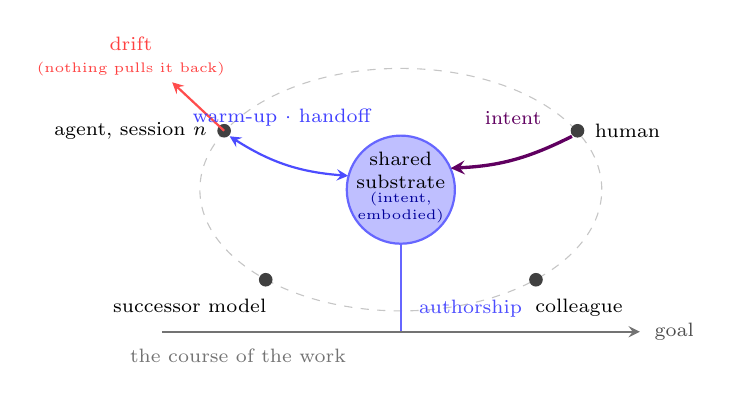
\begin{tikzpicture}[scale=0.88]
% orbit (dashed ellipse)
\draw[gray!45,dashed] (0,0) ellipse (2.9 and 1.75);
% pinned centroid
\filldraw[fill=blue!25,draw=blue!60,thick] (0,0) circle (0.78);
\node[font=\scriptsize,align=center] at (0,0.28) {shared\\substrate};
\node[font=\tiny,align=center,blue!60!black] at (0,-0.26) {(intent,\\embodied)};
% pin: post onto the course of the work (a rail toward the goal, not the ground)
\draw[thick,blue!60] (0,-0.78) -- (0,-2.05);
\draw[thick,blue!60] (-0.30,-2.05) -- (0.30,-2.05);
\node[font=\scriptsize,blue!70,anchor=west] at (0.12,-1.72) {authorship};
% the course
\draw[->,>=stealth,black!55,thick] (-3.45,-2.05) -- (3.45,-2.05);
\node[font=\scriptsize,black!70,anchor=west] at (3.52,-2.05) {goal};
\node[font=\scriptsize,black!55,anchor=north] at (-2.35,-2.16) {the course of the work};
% point masses on / near the orbit
\filldraw[black!75] (2.55,0.85) circle (0.09);
\node[font=\scriptsize,anchor=west] at (2.66,0.85) {human};
\filldraw[black!75] (-2.55,0.85) circle (0.09);
\node[font=\scriptsize,anchor=east] at (-2.66,0.85) {agent, session $n$};
\filldraw[black!75] (-1.95,-1.30) circle (0.09);
\node[font=\scriptsize,anchor=north east] at (-1.80,-1.44) {successor model};
\filldraw[black!75] (1.95,-1.30) circle (0.09);
\node[font=\scriptsize,anchor=north west] at (1.80,-1.44) {colleague};
% excursion (drift): agent drifting outward; nothing restores it
\draw[->,>=stealth,red!70,thick] (-2.55,0.85) -- (-3.30,1.55);
\node[font=\scriptsize,red!75,anchor=south east,align=center] at (-2.40,1.50) {drift\\{\tiny(nothing pulls it back)}};
% the session's coupling: it reads at warm-up, writes at handoff
\draw[<->,>=stealth,blue!70,thick] (-2.47,0.77) to[bend right=14] (-0.76,0.20);
\node[font=\scriptsize,blue!75,anchor=south,align=center] at (-1.72,0.78) {warm-up $\cdot$ handoff};
% the human's distinctive flow: authored intent, to the substrate boundary
\draw[->,>=stealth,violet!75!black,very thick] (2.47,0.77) to[bend left=12] (0.72,0.31);
\node[font=\scriptsize,violet!75!black,anchor=south] at (1.62,0.80) {intent};
\end{tikzpicture}
\caption{The pinned centroid. Participants in sustained work ---
human, agents, successive models, colleagues --- are noisy point
masses, and the arrows carry the asymmetry of the coupling. The
human's arrow deposits \emph{intent}: the substrate is that
intent, embodied. A session couples to the centroid by reading at
warm-up and writing at handoff; drift is the excursion of a
participant with nothing to pull it back; and a model swap moves a
point mass without moving the centroid. The pin is authorship, and
it fixes the centroid not to a place but to the course of the
work: what stays constant is reference, not position.}
\label{fig:centroid}
\end{figure}

The centroid names what the substrate does for the ensemble. It
does not yet say what the substrate \emph{is} to the participant
who originates the work, and that relation deserves to be stated
precisely, because it is the paper's real subject. Intent --- the
choice of what to build and why, the resolution of a trade-off,
the judgment that an option list is missing the one option that
matters --- is an \emph{event in a mind}. It occurs at a moment,
from a perspective, and then it is over. Work, by contrast, is
extended in time: it spans sessions, tools, models, and eventually
other minds. Unembodied intent has no duration, no location, and
no existence for anyone else --- including the operator's own
future self, who returns after a gap as, in every respect that
matters here, another participant.

The substrate is that event given a body. To embody an intent is
to convert it from something that \emph{happened} into something
that \emph{exists}, and existence here has exactly three
requirements: the embodied intent persists (storage), can be found
(address), and can be checked (an oracle appropriate to its
layer). The discipline's apparatus maps onto the three almost one
for one: version control and append-only records supply
persistence; stable identifiers and the inventory supply address;
contracts, budgets, and review supply checkability. The grades
matter because they fail separately. An intent that is merely
remembered dies with the session. An intent that is recorded
survives, but must be rediscovered to matter. An intent that is
addressable can be cited, tested, and built upon by participants
who never met its author. The discipline's central demand ---
deposit the choice once, at the layer where it belongs --- is the
demand that embodiment happen at the moment of authorship, rather
than be reconstructed later from its consequences. A musical score
stands in exactly this relation to a performance: not the music
and not the composer, but the composer's intent in durable,
addressable notation, from which any competent orchestra ---
including one assembled long after the composer --- can expand the
sound.

Read against this relation, the centroid image needs two glosses,
and it is honest to name them. First, a centre of mass is
democratic: it weights every mass alike. The substrate is not the
average of the ensemble's positions; it is the embodied intent the
ensemble reverts to, and intent flows into it from one direction
--- the human authors, the pipeline expands. The pin, in other
words, is authorship. Second, sustained work does not stand still.
The ensemble is going somewhere, and the substrate is what holds
it together on the way; so the centroid is pinned not to a place
but to the \emph{course} of the work
(Figure~\ref{fig:centroid}). The embodied intent rides toward the
goal with the ensemble orbiting it, drifting and reverting as
before, while it accretes the decisions the journey forces. What
the pin holds constant is not position but reference.

An older metaphor survives in the discipline's apparatus. The
artefact graph that realises the substrate is an \emph{atlas} ---
a set of maps at multiple scales, updated by successive surveyors
without losing fidelity, using conventions stable enough that
someone returning years later can still read them
(Figure~\ref{fig:atlas}). Maps shadow the territory at lower
fidelity than full understanding but with substantially higher
\emph{stability} --- and stability is what sustained work
requires, and what the unaided memory of any single mind, organic
or artificial, eventually fails to provide
(Figure~\ref{fig:drift}).

One more image, developed in \S\ref{sec:oracles}, completes the
set. Because the substrate is layered by abstraction --- the
shortest description at the top, progressively fuller detail
beneath --- it is a \emph{compressed representation} of the thing
being made: the small, dense, slow-changing description from
which agentic pipelines expand the full manifestation. What must
actually be written into it is only what no pipeline can
re-derive: the choices, the intent, the taste. That is the
discipline's purpose in one line --- \textbf{separate genuine
human creative input from cognitive load}. The creative input is
deposited once, at the layer where it belongs; the load --- the
re-explaining, the re-deriving, the bookkeeping --- is what the
substrate and its agents exist to absorb.

% --- F1 Drift Spectrum ---
\begin{figure}[t]
\centering
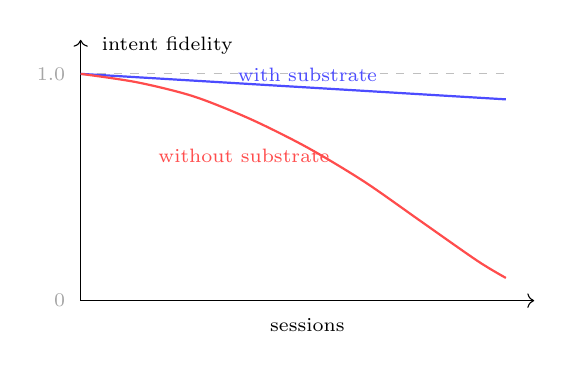
\begin{tikzpicture}[scale=0.72]
% axes
\draw[->] (0,0) -- (8,0);
\node[font=\scriptsize, anchor=north] at (4,-0.15) {sessions};
\draw[->] (0,0) -- (0,4.6);
\node[font=\scriptsize, anchor=west] at (0.2,4.5) {intent fidelity};
% baseline 1.0
\draw[gray!50, dashed] (0,4) -- (7.5,4);
\node[gray!70, font=\scriptsize, anchor=east] at (-0.1,4) {1.0};
\node[gray!70, font=\scriptsize, anchor=east] at (-0.1,0) {0};
% with substrate --- slow decay
\draw[blue!70, thick] (0,4) -- (7.5,3.55);
\node[blue!70, font=\scriptsize, anchor=south] at (4,3.7) {with substrate};
% without substrate --- fast decay
\draw[red!70, thick] plot[smooth] coordinates {(0,4) (1,3.85) (2,3.6) (3,3.2) (4,2.7) (5,2.1) (6,1.4) (7,0.7) (7.5,0.4)};
\node[red!70, font=\scriptsize, anchor=west] at (1.2,2.55) {without substrate};
\end{tikzpicture}
\caption{The drift spectrum. Without substrate discipline, intent
fidelity decays superlinearly across sessions; with substrate,
decay is bounded.}
\label{fig:drift}
\end{figure}

Two longer traditions deserve immediate credit. The cognitive-science
one has known for decades that cognition is not contained in heads
--- that it is \emph{distributed} across people, tools, and the
environment. Hutchins' analysis of ship navigation \citep{hutchins1995}
showed that the cognitive work of plotting a course is performed by a
system of people and instruments, not by any one mind.
\citet{scaife1996external} later distinguished between
\emph{internal} representations (in the head) and \emph{external}
representations (in the environment), showing how the latter can
radically reduce the cognitive load of complex tasks. The
software-engineering tradition has, for at least fifteen years,
externalised architectural decisions into append-only log entries
\citep{nygard2011adr} precisely to avoid the failure modes
catalogued in \S\ref{sec:failures}. Shared Substrate draws from
both. What it adds is the systematic application to a case the older
traditions could not have anticipated: where one of the
collaborators is a large language model whose every session begins,
in cognitive terms, with amnesia.

What follows is shaped by that observation. AI's most discussed
limitations on long-horizon work --- drift, phantom decisions,
restart cost --- are best understood as substrate failures rather
than model failures, and respond to substrate-level interventions
far more reliably than to model-level scaling. The discipline that
addresses them is not new; it is recovered, made explicit, and
applied. And the discipline is fundamentally human in its
\emph{governance}: intent, decisions of consequence, scope, and
voice remain with the person who cultivates it. Its
\emph{execution}, by contrast, is progressively delegable to the
agents themselves (\S\ref{sec:governance}) --- the same tools whose
limitations motivate the practice can be enlisted to maintain the
substrate that compensates for those limitations. AI's limitations
motivate the practice. Cognitive science legitimises it.
Human-governed, agent-executed practice carries it out. This
matters, because it means the discipline survives across model
generations: the governance schema is durable while the execution
layer evolves with the tooling.

The structure of what follows is straightforward.
\S\ref{sec:failures} catalogues the failure modes the discipline
addresses and situates them against a genuinely contested empirical
record. \S\ref{sec:foundations} traces the foundations from which
it draws. \S\ref{sec:discipline} specifies the discipline itself.
\S\ref{sec:oracles} pairs each abstraction layer with a
representation formalism and a verification oracle, and argues
that observability of the work's state is what closes the agent's
feedback loop. \S\ref{sec:governance} specifies the human-governance /
agent-execution division of labour and its adoption stack.
\S\ref{sec:synthesis} maps each element of the discipline to the
cognitive principle that grounds it, the failure mode it mitigates,
and the layer that automates it. \S\ref{sec:example} shows the
discipline in flight on two worked examples --- one greenfield,
one brownfield. \S\ref{sec:practice}--\S\ref{sec:limits} discuss
cost and the honest limits of the practice. \S\ref{sec:close}
closes.

\paragraph{Provenance.} The discipline articulated here was not
invented for this paper, nor co-developed with an AI agent in the
writing of it. It is a long-running reflection of the author
across many domains and many years --- a habit of thought and
work shaped by experience well outside the AI context, applied to
research, to engineering, and to sustained intellectual work of
several kinds. Books, lab notebooks, scientific notation, version
control, architectural decision records: each generation finds
apparatus for stabilising thought across time and distributing it
across minds, and the author has cultivated such apparatus, in
one form or another, on every complex project worth sustaining.
What working with current-generation language models on complex,
multi-session projects did was sharpen the apparatus into
something articulable: every implicit affordance of human-only
work became an explicit artefact when the collaborator was an
agent without persistent memory, and the elements of the
discipline became visible in a way they had not been before. This
paper names what was already there. The discipline applies
wherever sustained complex work crosses many sessions, decisions,
or abstraction layers --- not only where one of the collaborators
is an AI; collaboration with AI is what most recently made the
discipline's elements demand explicit articulation, and gave us
the occasion to name them. Acknowledgements at the end credit the
AI's specific role in helping draft and stress-test that
articulation.

% =====================================================================
\section{What We Observe When Substrate is Absent}
\label{sec:failures}
% =====================================================================

The motivating phenomena are not theoretical. They are what one comes
to see when collaborating with a large language model on any
sufficiently complex task without substrate discipline. The names
below are ours; the phenomena are widely reported across the
engineering community and increasingly studied formally
\citep{liu2024lostmiddle, park2023generativeagents, packer2024memgpt}.
Each is described from the inside --- what one sees, what one feels,
what fails.

\subsection{Context-window saturation}
Every session is bounded by a context window. Even with windows in
the hundreds of thousands or millions of tokens, the working set of
a long project --- accumulated decisions, terminology, partial
designs, prior versions --- outgrows the window faster than capacity
grows. The symptom is a creeping reluctance to introduce new
context; a sense of crowding; an instinct to compress prior content
into ever-shorter summaries. Each compression discards material the
next subtask might have needed. Capacity addresses the
\emph{amount} of state attended to at once, not the \emph{amount}
the project has accumulated. These are different quantities, and
only the second grows superlinearly with project complexity.

\subsection{Lost-in-the-middle and attention dilution}
When relevant content does fit in the window, it is not equally
accessible across positions. The literature on long-context
retrieval consistently finds that information placed in the middle
of a long context is retrieved less reliably than information at the
start or end \citep{liu2024lostmiddle}. Felt from the human side,
this is inconsistent recall: a fact stated three messages ago is
honoured; a fact stated thirty messages ago is forgotten or
contradicted, even though it remains technically present.
Compounding this, every additional irrelevant token dilutes
attention that could have been spent on the relevant ones. The
agent is the same; the substrate is now noisier.

\subsection{Drift across iterations}
Without an external reference for the project's settled state, each
iteration is built atop the last iteration's reconstruction of it.
Small reconstruction errors compound. After enough iterations, the
running understanding has drifted measurably from any historical
anchor. The phenomenon shows up as a sense of ``we already decided
that, didn't we?'' with the answer increasingly uncertain; or as a
drift in terminology, where a term used precisely in week one is
used loosely by week three; or as the gentle reinvention of
solutions previously rejected for reasons no longer remembered.

\subsection{Phantom decisions}
The most consequential failure mode. Asked ``did we decide X?'',
the agent answers based on a probabilistic reconstruction from
available context --- it cannot reliably distinguish ``this was
decided'' from ``this was discussed and was a plausible thing to
decide''. Without an external decision register, the agent
\emph{will confidently confabulate}, citing reasoning that never
occurred and conclusions never reached. The human side often
discovers this only when the phantom decision contradicts a real
one; sometimes only when implementation reveals the inconsistency.
The risk is most acute precisely on the decisions that matter most
--- load-bearing choices made early and referred to often.

\subsection{Reference rot}
In informal practice, references to prior work are by file path or
paraphrase: ``in the requirements doc, the section about latency''.
Reorganise the file or refactor the section, and every such
reference becomes stale. The agent, asked to ``see the latency
section'', produces a plausible reconstruction of what such a
section \emph{would have said}. The human side cannot easily
distinguish reconstructed content from quoted content. References
that were meaningful in week one are increasingly noise by week
three.

\subsection{Restart cost}
Every new session begins with whatever substrate can be mustered
from memory and immediately-available files. Without a stable
warm-up substrate, the early minutes of every session go into
re-explaining context: who is doing what, what is being built,
what was decided last week, what the open questions are. The cost
is borne on one side as fatigue and on the other as crowded
context. In aggregate, a project that requires twenty sessions
pays the restart cost twenty times.

\subsection{Decided versus considered confusion}
In a chat transcript there is no intrinsic distinction between
``this was decided'' and ``this was considered''. Both look like
prose. The human side relies on memory or implicit context to
distinguish them. The agent, lacking that mental annotation, treats
both as equivalent input. Over time, \emph{considered} options
accumulate in the running context with the same status as
\emph{decided} ones, and the agent begins to act as if they were
settled. Contraries emerge silently, often resolved by the next
iteration's reconstruction in whichever direction the immediate
context happens to favour.

\subsection*{A common shape}
These seven failure modes share a single shape. None is a property
of any particular model; each is a property of \emph{unsubstrated
collaboration}. Bigger models with longer context windows shift
the magnitude of each --- the threshold at which it appears, the
rate at which it compounds --- without changing the underlying
topology. Each admits a substrate-level intervention more reliable
than any model-level fix. The remainder of the paper specifies
those interventions and grounds them in the cognitive-science and
software-engineering traditions that have, in different idioms,
addressed precisely these failure modes for decades.

\subsection*{The contested empirical record}
The failure modes above are felt from the inside; their aggregate
cost is now visible from the outside, and the picture is genuinely
contested. The most methodologically careful randomised controlled
trial to date \citep{becker2025metr} --- sixteen experienced
open-source developers, 246 real tasks on mature repositories they
knew well --- found that access to early-2025 AI tooling
\emph{increased} task completion time by 19\%, while the same
developers had forecast a 24\% speed-up and, even after the
experiment, still believed the tools had made them about 20\%
faster. Field experiments across 4{,}867 developers
\citep{cui2026effects} found the opposite sign: a 26\% increase in
completed tasks, concentrated among less experienced developers.
A controlled greenfield task \citep{peng2023copilot} found a 56\%
speed-up. These results are not mutually inconsistent; they are
measurements of differently configured couplings.
\citet{farrag2026paradox} reconciles them through three
moderators: the abstraction level of the task, the maturity of the
codebase, and the experience of the operator.

We read this record as the strongest available motivation for
substrate discipline, for two reasons. First, the calibration
failure in \citet{becker2025metr} --- developers who are slowed
down while confidently believing they are sped up --- means felt
productivity cannot be trusted as the measure of a human--AI
coupling; only externalised, inspectable state can be
(\S\ref{sec:oracles} proposes the replacement measurand). Second, the
moderators that determine which regime a coupling lands in are
precisely substrate-adjacent variables: what the project's
accumulated context is, how it is represented, and at what
abstraction level the human operates. The discipline of this paper
is an intervention on those moderators, and that claim is
falsifiable: if practised substrate discipline does not move
experienced operators on mature projects out of the slowdown
regime, the thesis of this paper fails.

% =====================================================================
\section{What We Inherit: Foundations}
\label{sec:foundations}
% =====================================================================

The discipline did not emerge from a vacuum. Three traditions ---
none of which uses the term \emph{Shared Substrate} --- converge
on its elements. The cognitive-science tradition supplies the
deepest framing; the software-engineering tradition supplies hard-won
precedent; the agentic-AI literature supplies the contemporary
motivation and a small but growing apparatus.

\subsection{Cognitive science}

What Shared Substrate asks of an operator is not foreign to
humans --- it is what humans do when they think well at scale, made
explicit and applied to a new collaborator.

\citet{hutchins1995} argued in \emph{Cognition in the Wild} that
cognitive work is not contained in heads. The plot of a ship's
position is computed by a system: navigators, charts, plotting
tables, instrument readings, written-down conventions. No one mind
holds the whole computation. The chart is not a record of the
navigator's thinking --- it is part of the thinking. Shared
Substrate is a particular distribution: the artefact graph is
part of the project's cognition, not a passive record of it.

\citet{scaife1996external} sharpened the distinction between
internal representations (mental models held in working memory) and
external representations (graphics, tables, diagrams, documents).
External representations radically alter what cognitive operations
are possible: certain reasoning steps are easy on a diagram and hard
in the head. The complexity of a project's accumulated state is
not a quantity to be carried internally; it is a structure to be
externalised. \citet{risko2016offloading} corroborate this
empirically: people routinely offload to calendars, lists, sketches,
GPS devices when cognitive demands rise, and the offloading
demonstrably frees working-memory resources for harder operations.

The need rests on hard capacity limits. \citet{baddeley1992wm}
established the architecture of working memory;
\citet{cowan2001magical} placed the realistic capacity at roughly
four chunks, sharpening \citet{miller1956magical}'s earlier
estimate. Whatever the exact number, the order of magnitude is
small. A project with eighty open considerations is not held in any
one mind. It must live in the substrate.

\citet{bartlett1932remembering} showed that memory is reconstructive:
recall is shaped by pre-organised \emph{schemata} that guide
pattern-completion. An LLM asked ``did we decide X?'' performs an
analogous reconstructive process --- and like human memory, it can
confabulate plausibly when the schema fits. The remedy is the same
remedy human cognition has used for millennia: produce a stable
external trace that can be consulted instead of reconstructed.

\citet{marr1982vision} formalised what software engineers and
cognitive scientists have repeatedly rediscovered: complex
information-processing problems decompose into distinct levels of
analysis --- computational, algorithmic, implementational. Each
level has its own questions and its own appropriate language.
Shared Substrate's hierarchy of abstraction layers
(Figure~\ref{fig:hierarchy}) is a Marr-shaped commitment. The brain
itself, in current accounts \citep{friston2010fep, clark2013whatever},
is a hierarchical predictive system; sustained inference is
hierarchical because the flat alternative is intractable.

\citet{star1989boundary} introduced \emph{boundary objects}:
artefacts that mean different things to different communities but
enable coordination because they are robust enough to survive the
variation. The artefacts of Shared Substrate are boundary
objects between human and AI agent: each reads them with different
prior contexts, but both can refer to the same artefact and update
it without confusion. The stable identifier --- KB-N, ADR-N, OQ-N
--- is the canonical boundary object.

\citet{sweller1988cognitive} formalised cognitive load theory:
mental resources are spent on \emph{intrinsic} (what the material
demands), \emph{extraneous} (what bad presentation imposes), and
\emph{germane} (what supports schema construction) load. Substrate
discipline imposes intrinsic load (the discipline must be held in
mind) but substantially reduces extraneous load (no more
re-explaining what was decided) and increases germane load (the
substrate makes patterns visible). Above a threshold of project
complexity the trade is favourable; \S\ref{sec:practice} addresses
where that threshold lies.

\subsection{Software engineering}

The failure modes catalogued in \S\ref{sec:failures} are not new;
they have visited every team that has built complex software for
more than a few months, and the tradition's solutions have been
recurrent enough to deserve names.

\citet{nygard2011adr}'s Architectural Decision Records made the
single most consequential of those solutions explicit. An ADR is a
short append-only document recording one architectural decision, its
context, its rationale, the alternatives considered, and its
consequences. The crucial feature is the discipline of appending: an
ADR is never edited; reversal happens via a new ADR that supersedes
the old. The reasoning trail is preserved, not just the current
answer. Fifteen years of practice across many organisations have
shown the pattern resists rot in ways ad-hoc design notes do not.
Shared Substrate adopts ADRs unmodified.

\citet{cockburn2005hexagonal}'s hexagonal architecture (Ports and
Adapters) makes a related move at the architectural level: the
domain depends only on abstract \emph{ports}; concrete adapters
implement those ports. The discipline produces clean separability:
the domain can be tested without touching infrastructure, and
adapters can be swapped without disturbing the domain. The analogue
at the substrate level is the separation between artefacts of
different kinds, and the discipline of cross-referencing only via
stable identifiers.

\citet{hunt1999pragmatic} crystallised \emph{Don't Repeat Yourself}
(DRY): every piece of knowledge must have a single, unambiguous,
authoritative representation within a system. DRY is usually
discussed at the level of code, but the principle generalises. In
Shared Substrate, every fact has one home; everywhere else
references it by id. Duplicate prose is treated as a bug --- the
same way duplicate code is. The duplicates will diverge, the
divergence will be noticed late, and the cost of reconciling will
exceed the cost of the original abstraction.

\citet{candea2003crashonly} proposed crash-only software: a program
designed so that the only way to stop it is to crash, and the only
way to start it is from a cold-start replay. The benefit is that
the recovery path is the only path, and is therefore exercised on
every restart rather than only in disasters. Shared Substrate
adopts the same logic: every session begins by reading the artefact
graph from disk, regardless of whether the previous session ended
cleanly or crashed. There is no separate ``warm restart'' path.

These four practices --- ADRs, hexagonal separation, DRY,
crash-only --- were developed independently for different software
problems. Their convergence on a recognisably common shape --- a
disciplined, externalised, append-only, sparingly cross-referenced
substrate that survives reorganisation --- is itself evidence that
the discipline is a recurrent solution. Shared Substrate
names that shape and applies it where it has so far been least
practised.

\subsection{Agentic AI}

The agentic-AI tradition is the youngest and supplies the
contemporary motivation. AI systems built to operate over long
horizons --- to research, plan, browse, simulate --- confront the
substrate problem acutely: a context window is finite, the project
is not.

\citet{lewis2020rag} introduced retrieval-augmented generation: rather
than packing all relevant context into the prompt, retrieve the
relevant pieces from an external store at query time. RAG is now the
dominant pattern for grounding LLM responses in specific knowledge
bases. From the substrate perspective, RAG is a partial
answer: it solves ``how to bring relevant context to the agent at
the moment of need'' but not ``how to maintain that context's
coherence as the project evolves''. The substrate retrieved into
the agent's working context is only as good as the substrate
sitting at rest.

\citet{packer2024memgpt} pushed harder, treating the LLM as the
kernel of an operating system with explicit memory-management
primitives --- paging, hierarchical buffers, persistent storage.
The MemGPT analogue of working memory and long-term memory mirrors
the cognitive-science distinction between internal and external
representations \citep{scaife1996external}. Shared Substrate's
session warm-up is a coarse version of MemGPT-style paging,
performed by a human operator at the start of work rather than
continuously by the model.

\citet{park2023generativeagents} demonstrated that long-running
simulated agents required explicit memory and reflection machinery
to behave coherently across simulated days. They combined a flat
memory store with retrieval and reflective summarisation. The
simulated agents' need for these mechanisms is the same need an
operator has when collaborating with an LLM over many sessions,
and the same set of solutions emerges in different idioms.

\citet{shinn2023reflexion} showed that agents which reflect verbally
on their own behaviour --- generating critiques and revisions
before retrying --- outperform agents that do not. The analogue at
the substrate level is the editing protocol: the discipline mandates
a pre-edit reflection (READ, IDENTIFY SSOT, IMPACT-CHECK) before
changes are made. Reflection is not optional; it is the protocol.

\citet{bai2022constitutional} proposed Constitutional AI: encoding a
small set of explicit rules the agent self-applies during
generation. The constitution sits outside any single response and
governs all of them. Shared Substrate's edit protocol is a
constitution at the methodological level --- explicit rules an
operator self-applies whenever touching the substrate.

The convergence has since become structural. Agentic-memory
systems now organise an agent's persistent state as networks of
atomic, interlinked, evolving notes --- A-MEM's Zettelkasten-style
memory is explicit about the lineage \citep{xu2025amem} --- and
hierarchical and graph-native memory architectures recapitulate,
in system design, the artefact-graph shape this paper specifies as
practice. The convergence extends to the tooling vendors: by
2025--26, nearly every commercially shipping AI coding harness had
independently adopted a small auto-loaded project-root instruction
file as its session entry point. Operators cultivating a
discipline, researchers designing memory systems, and vendors
shipping harnesses arrived at structurally similar substrate
solutions without coordinating --- the same convergence argument
made above for the software-engineering tradition, and the same
kind of evidence that the shape is a recurrent solution rather
than a stylistic preference.

The agentic-AI literature is converging from many directions on a
common conclusion: long-horizon AI work requires explicit external
state, retrieval and pre-fetch, reflection, and rules. Shared
Substrate offers no new component over this literature; it offers
a methodology that integrates them at the level the operator
inhabits --- and, in \S\ref{sec:governance}, a governance schema
for progressively delegating substrate execution to these very
systems.

% =====================================================================
\section{Shared Substrate: The Discipline}
\label{sec:discipline}
% =====================================================================

The discipline of Shared Substrate is specified by six
artefact categories, a set of stable cross-referencing conventions,
an explicit status lifecycle, an edit protocol, propagation rules
across an explicit hierarchy of abstraction layers, an anti-pattern
catalogue, and a session protocol. Each piece is modest in itself;
the leverage comes from their combination
(Figures~\ref{fig:hierarchy}, \ref{fig:atlas}).

A note on execution before the specification. What follows
describes the discipline in its fully-manual baseline form ---
every step performed by the operator. \S\ref{sec:governance}
specifies how execution is progressively delegated to agents;
delegation changes \emph{who performs} each step, never what the
step is or who is accountable for it.

% --- F2 Hierarchy of Maps ---
\begin{figure}[t]
\centering
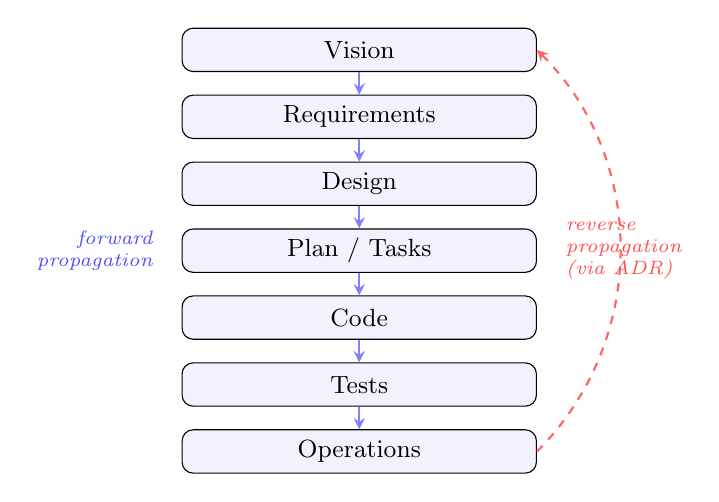
\begin{tikzpicture}[
    layer/.style={draw,rounded corners,fill=blue!5,minimum width=4.5cm,minimum height=0.55cm,anchor=center,font=\small},
]
\node[layer] (vision)   at (0,5.4) {Vision};
\node[layer] (req)      at (0,4.55) {Requirements};
\node[layer] (design)   at (0,3.7) {Design};
\node[layer] (plan)     at (0,2.85) {Plan / Tasks};
\node[layer] (code)     at (0,2.0) {Code};
\node[layer] (tests)    at (0,1.15) {Tests};
\node[layer] (ops)      at (0,0.3) {Operations};
\foreach \i/\j in {vision/req,req/design,design/plan,plan/code,code/tests,tests/ops}
  \draw[->,>=stealth,thick,blue!50] (\i.south) -- (\j.north);
\draw[<-,>=stealth,thick,dashed,red!60] (vision.east) to[bend left=45] (ops.east);
\node[anchor=west,red!70,font=\scriptsize\itshape,align=left] at (2.5,2.85) {reverse\\propagation\\(via ADR)};
\node[anchor=east,blue!70,font=\scriptsize\itshape,align=right] at (-2.5,2.85) {forward\\propagation};
\end{tikzpicture}
\caption{The hierarchy of maps. Each layer is a distinct
representation; forward propagation cascades changes downward;
reverse propagation requires deliberate revision via Decision
Records.}
\label{fig:hierarchy}
\end{figure}

% --- F3 Atlas ---
\begin{figure*}[t]
\centering
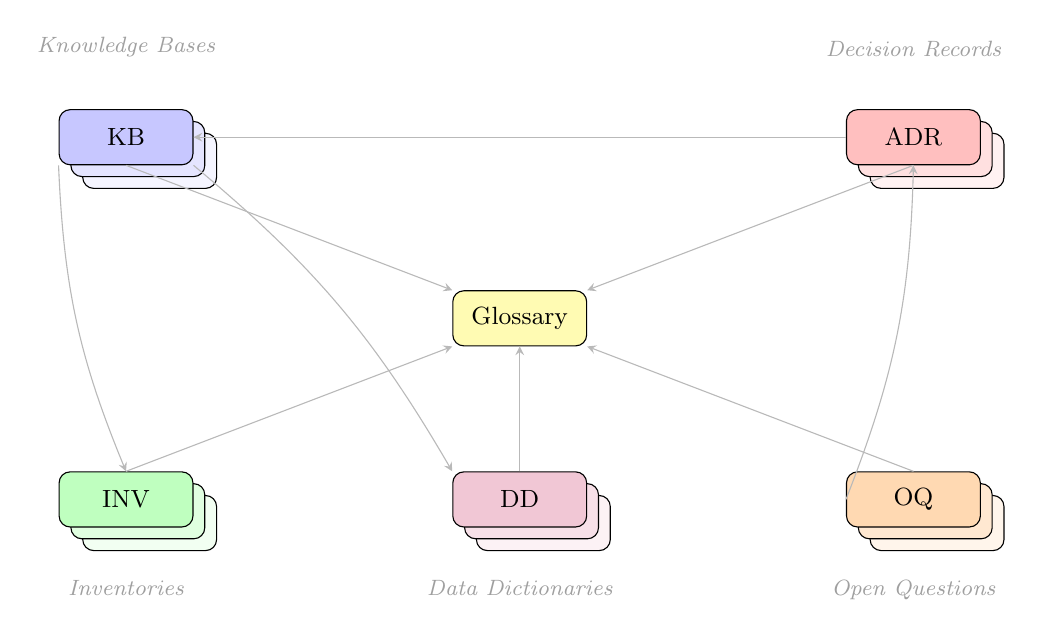
\begin{tikzpicture}[
    every node/.style={font=\small},
    artifact/.style={draw,rounded corners,minimum width=1.7cm,minimum height=0.7cm},
    arrow/.style={->,>=stealth,gray!55},
]
% Central glossary --- semantic anchor
\node[artifact,fill=yellow!30] (gloss) at (0,0) {Glossary};

% --- Stacked-box pattern: two shadow boxes behind each labelled box,
%     suggesting multiplicity (``and many more'') without committing
%     to specific numbering.

% KB stack (top-left)
\node[artifact,fill=blue!4]  at ($(-5.0,2.3)+(0.30,-0.30)$) {};
\node[artifact,fill=blue!10] at ($(-5.0,2.3)+(0.15,-0.15)$) {};
\node[artifact,fill=blue!22] (KB) at (-5.0,2.3) {KB};

% ADR stack (top-right)
\node[artifact,fill=red!5]  at ($(5.0,2.3)+(0.30,-0.30)$) {};
\node[artifact,fill=red!12] at ($(5.0,2.3)+(0.15,-0.15)$) {};
\node[artifact,fill=red!25] (ADR) at (5.0,2.3) {ADR};

% INV stack (bottom-left)
\node[artifact,fill=green!5]  at ($(-5.0,-2.3)+(0.30,-0.30)$) {};
\node[artifact,fill=green!12] at ($(-5.0,-2.3)+(0.15,-0.15)$) {};
\node[artifact,fill=green!25] (INV) at (-5.0,-2.3) {INV};

% DD stack (bottom-centre)
\node[artifact,fill=purple!5]  at ($(0,-2.3)+(0.30,-0.30)$) {};
\node[artifact,fill=purple!12] at ($(0,-2.3)+(0.15,-0.15)$) {};
\node[artifact,fill=purple!22] (DD) at (0,-2.3) {DD};

% OQ stack (bottom-right)
\node[artifact,fill=orange!8]  at ($(5.0,-2.3)+(0.30,-0.30)$) {};
\node[artifact,fill=orange!18] at ($(5.0,-2.3)+(0.15,-0.15)$) {};
\node[artifact,fill=orange!30] (OQ) at (5.0,-2.3) {OQ};

% --- References (illustrative, not exhaustive)
% Every category references the glossary
\draw[arrow] (KB.south)  -- (gloss.north west);
\draw[arrow] (ADR.south) -- (gloss.north east);
\draw[arrow] (INV.north) -- (gloss.south west);
\draw[arrow] (DD.north)  -- (gloss.south);
\draw[arrow] (OQ.north)  -- (gloss.south east);
% Selected cross-category cross-references
\draw[arrow] (ADR.west) -- (KB.east);
\draw[arrow] (KB.south west) to[bend right=10] (INV.north);
\draw[arrow] (KB.south east) to[bend left=10]  (DD.north west);
\draw[arrow] (OQ.west) to[bend right=10] (ADR.south);

% Annotations
\node[font=\footnotesize\itshape,gray!75,anchor=south] at (-5,3.2) {Knowledge Bases};
\node[font=\footnotesize\itshape,gray!75,anchor=south] at (5,3.2)  {Decision Records};
\node[font=\footnotesize\itshape,gray!75,anchor=north] at (-5,-3.2) {Inventories};
\node[font=\footnotesize\itshape,gray!75,anchor=north] at (0,-3.2)  {Data Dictionaries};
\node[font=\footnotesize\itshape,gray!75,anchor=north] at (5,-3.2)  {Open Questions};
\end{tikzpicture}
\caption{The atlas. An artefact graph linking Knowledge Bases,
Inventories, Data Dictionaries, Decision Records, and Open
Questions, with the Glossary as central semantic anchor. Stacked
boxes indicate that each category typically contains many
artefacts; arrows are illustrative cross-references, not
exhaustive. Cross-references use stable identifiers that survive
reorganisation of the file tree.}
\label{fig:atlas}
\end{figure*}

\subsection{Six artefact categories}

The substrate is composed of six kinds of artefact. Each kind has
explicit semantics, an explicit format, and explicit rules about
who is allowed to change it and when. The taxonomy is deliberately
small: more categories would invite ambiguity about which one a
given piece of content belongs to.

\textbf{Knowledge Bases (KB-N)} hold durable, slow-changing facts
about the world the project operates in --- the constraints of an
external API, the regulatory environment, the assumptions of an
underlying scientific tradition. KBs cite external sources with
access dates and are reviewed at a cadence proportional to how
fast their underlying world changes.

\textbf{Inventories (INV-N)} are exhaustive lists in well-defined
categories: every supported order type, every emitted metric, every
returnable error code. Where a KB explains, an Inventory enumerates.
Inventories are designed to be machine-checkable: an automated test
should be able to assert that every metric in the code is in the
inventory and every entry in the inventory is in the code.

\textbf{Data Dictionaries (DD-N)} are schemas: every field of every
domain object, with type, semantics, invariants, and example. A
Data Dictionary is the artefact a tool can validate against. It is
also the artefact that makes interface boundaries explicit: two
components agree on a Data Dictionary, and the dictionary becomes
the contract.

\textbf{Architectural Decision Records (ADR-N)} record decisions, in
the sense of \citet{nygard2011adr}: a context, a decision, the
alternatives considered, the consequences. ADRs are append-only.
Reversal happens via a new ADR with a supersedes link to the old.
The reasoning trail is preserved.

\textbf{Open Questions (OQ-N)} are the dual of decisions:
deliberately unresolved questions, with target resolution dates,
options under consideration, and resolution criteria. OQs prevent
the silent slide from ``we are deliberately not deciding this yet''
into ``we forgot we needed to decide this''. Once an OQ is resolved
the resolution moves to an ADR; the OQ status updates to
\textsc{resolved-by-adr-n}; both records persist.

\textbf{Glossary} is the singular authority on terminology. Every
term used twice in the substrate with the same meaning belongs in
the glossary. If two artefacts disagree on a term's meaning, the
glossary wins or both are wrong; conversation is required. The
glossary is the substrate's semantic anchor.

The categories partition the substrate. Every piece of project
knowledge belongs to exactly one of the six. The categories also
have characteristic update cadences --- KBs change rarely,
Inventories change with each new feature, ADRs are append-only, OQs
accumulate and resolve, the Glossary grows and stabilises. The
differential cadence is itself useful; it tells the operator
what kind of artefact they are looking at without reading the
content.

\subsection{Stable identifiers and the cross-reference graph}

Every artefact carries a stable identifier of the form
$\langle$category-letter$\rangle$-$\langle$number$\rangle$: KB-1,
INV-4, DD-7, ADR-12, OQ-23. Identifiers are assigned monotonically
and never reused. Cross-references throughout the substrate use
these identifiers --- never file paths, never section numbers,
never paraphrases.

The reason is simple. File paths reorganise; section numbers shift
on insertion; paraphrases drift in meaning. Each is a route to
reference rot. A stable identifier survives reorganisation: KB-3
remains KB-3 whether its file is at \texttt{docs/kb/} or
\texttt{kb/} or has been moved into a subdirectory. The
identifier-based cross-reference is a boundary object
\citep{star1989boundary} between today's substrate layout and
tomorrow's: both layouts agree on what KB-3 is, even though they
agree on nothing else about where it lives.

Every artefact also lists the artefacts it depends on
(\texttt{depends\_on}) and the artefacts that reference it
(\texttt{referenced\_by}). Together these turn the substrate into a
navigable graph. The graph supports impact analysis: before editing
KB-3, the operator walks \texttt{KB-3.referenced\_by} and
reviews each downstream artefact. The graph supports orphan
detection: an artefact whose \texttt{referenced\_by} stays empty
for more than one milestone is a candidate for retirement. The
graph supports cycle detection: two artefacts that depend on each
other suggest a missing third artefact that should own the shared
content.

The atlas (Figure~\ref{fig:atlas}) is a partial picture of the
graph at a moment in time. The full graph is implicit in the
\texttt{depends\_on} and \texttt{referenced\_by} fields of every
artefact, and could be rendered automatically by tooling
(\S\ref{sec:governance}).

\subsection{Status lifecycle}

Every artefact has a status, drawn from five values
(Figure~\ref{fig:status}): \textsc{missing} (named in the inventory
but no file yet), \textsc{draft} (file exists, content incomplete
or not yet reviewed), \textsc{stable} (content current and complete
to the level required), \textsc{stale} (content was once stable
but the underlying world has changed or an upstream artefact has
changed since last review), and \textsc{deprecated} (superseded;
kept for history, must not be referenced by new work).

% --- F4 Status Lifecycle ---
\begin{figure}[t]
\centering
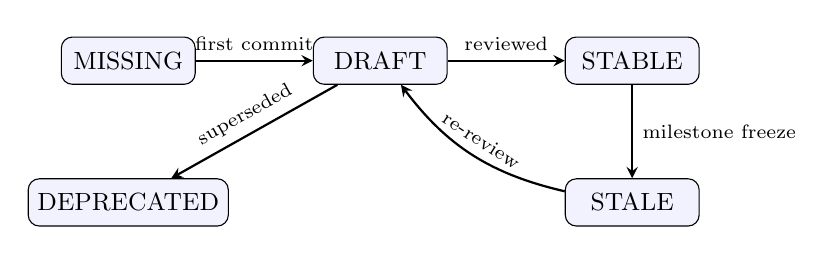
\begin{tikzpicture}[
    state/.style={draw,rounded corners,minimum width=1.7cm,minimum height=0.6cm,fill=blue!5,font=\small},
    arrow/.style={->,>=stealth,thick},
]
\node[state] (miss)    at (-3.2,3) {MISSING};
\node[state] (draft)   at (0,3) {DRAFT};
\node[state] (stab)    at (3.2,3) {STABLE};
\node[state] (stale)   at (3.2,1.2) {STALE};
\node[state] (dep)     at (-3.2,1.2) {DEPRECATED};

\draw[arrow] (miss) -- node[above,font=\scriptsize] {first commit} (draft);
\draw[arrow] (draft) -- node[above,font=\scriptsize] {reviewed} (stab);
\draw[arrow] (stab) -- node[right,font=\scriptsize] {milestone freeze} (stale);
\draw[arrow] (stale) to[bend left=20] node[above,font=\scriptsize,sloped] {re-review} (draft);
\draw[arrow] (draft) -- node[above,font=\scriptsize,sloped] {superseded} (dep);
\end{tikzpicture}
\caption{Status lifecycle. Transitions are explicit and triggered;
no artefact silently changes state.}
\label{fig:status}
\end{figure}

Each transition has an explicit trigger. \textsc{missing} to
\textsc{draft} is the first content commit. \textsc{draft} to
\textsc{stable} is owner review with completeness check.
\textsc{stable} to \textsc{stale} is either a milestone-freeze gate
(if the artefact has not been reviewed by the gate, status
auto-degrades) or a propagation event from an upstream artefact
that changed substantively. \textsc{stale} to \textsc{stable} is
re-review. Anything to \textsc{deprecated} is supersedure.

The discipline is that the status field is mandatory and accurate.
``Eventually consistent'' is treated as a bug, not a feature: if
two artefacts disagree, the disagreement is logged with a target
reconciliation date, not silently tolerated. The same applies
between an artefact's stated status and its actual freshness --- a
\textsc{stable} artefact with a six-month-old review date during a
fast-moving project is not stable; it is stale, and should be
labelled accordingly.

The status field, combined with the cadence rules from \S4.1, gives
the operator a quick estimate of the substrate's overall
health. A substrate with most artefacts in \textsc{stable} or
\textsc{draft} and few in \textsc{stale} is in good shape. A
substrate with many \textsc{stale} or \textsc{missing} artefacts is
signalling that the operator has out-grown the substrate or
under-tended it.

\subsection{The edit protocol}

Every change to the substrate follows a sequence
(Figure~\ref{fig:editproto}).

% --- F5 Edit Protocol ---
\begin{figure}[t]
\centering
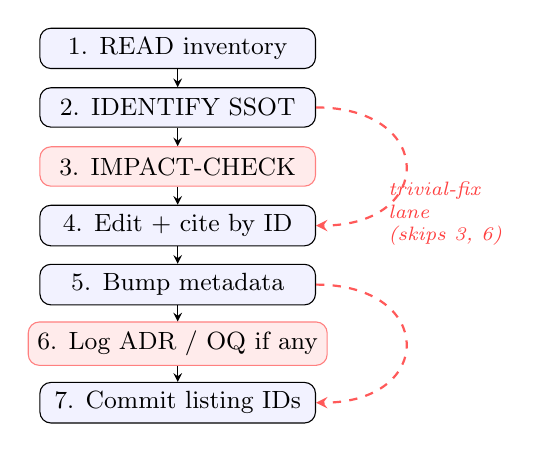
\begin{tikzpicture}[
    pstep/.style={draw,rounded corners,minimum width=3.5cm,minimum height=0.5cm,font=\small,fill=blue!5},
    skipbox/.style={draw,rounded corners,minimum width=3.5cm,minimum height=0.5cm,font=\small,fill=red!8,draw=red!50},
    arrow/.style={->,>=stealth},
    bypass/.style={->,>=stealth,red!65,dashed,thick},
]
\node[pstep]   (read)   at (0,5.6)  {1. READ inventory};
\node[pstep]   (id)     at (0,4.85) {2. IDENTIFY SSOT};
\node[skipbox] (impact) at (0,4.10) {3. IMPACT-CHECK};
\node[pstep]   (edit)   at (0,3.35) {4. Edit + cite by ID};
\node[pstep]   (bump)   at (0,2.60) {5. Bump metadata};
\node[skipbox] (decide) at (0,1.85) {6. Log ADR / OQ if any};
\node[pstep]   (commit) at (0,1.10) {7. Commit listing IDs};

% Main path (top-down through all steps)
\draw[arrow] (read)   -- (id);
\draw[arrow] (id)     -- (impact);
\draw[arrow] (impact) -- (edit);
\draw[arrow] (edit)   -- (bump);
\draw[arrow] (bump)   -- (decide);
\draw[arrow] (decide) -- (commit);

% Trivial-fix lane: red dashed bypasses skipping steps 3 and 6
\draw[bypass] (id.east)   to[out=0,in=0,looseness=2.6] (edit.east);
\draw[bypass] (bump.east) to[out=0,in=0,looseness=2.6] (commit.east);

% Annotation
\node[font=\scriptsize\itshape,red!75,anchor=west,align=left]
  at (2.55,3.5) {trivial-fix\\lane\\(skips 3, 6)};
\end{tikzpicture}
\caption{The edit protocol. The main path runs top-down through
all seven steps. The trivial-fix lane (red dashed arrows) bypasses
\textsc{impact-check} (step 3) and decision-logging (step 6),
which are the steps that do not apply to typos and
mechanical fixes. Steps 4, 5, and 7 always run.}
\label{fig:editproto}
\end{figure}

Before the edit: \textbf{READ} the inventory to confirm the artefact
exists at the expected status; \textbf{IDENTIFY} which artefact owns
the fact you intend to change (the Single Source of Truth, in the
language of \citet{hunt1999pragmatic}); and \textbf{IMPACT-CHECK} by
walking the artefact's \texttt{referenced\_by} list to identify
downstream artefacts that may need to update.

During the edit: touch the minimum surface needed. Use stable
identifiers in cross-references --- never file paths, never
paraphrases. Where you find yourself paraphrasing content from
another artefact, replace the paraphrase with a citation. Where you
find that the same fact lives in two artefacts, consolidate.

After the edit: bump \texttt{last\_reviewed}; if the change is
substantive, bump \texttt{version}; if status changes, update the
inventory in the same commit. If the edit reflects a decision among
alternatives, write the corresponding ADR in the same commit. If
the edit raises a question that cannot be resolved in line, write
the corresponding OQ. Commit messages list every artefact touched,
by stable identifier.

\paragraph{The trivial-fix lane.} A protocol that imposes the full
sequence on every typo is a protocol that gets bypassed. A
trivial-fix lane is built in: typos, formatting, broken markdown,
link fixes that do not change meaning skip the IMPACT-CHECK and the
decision-logging steps. The \texttt{last\_reviewed} field still
bumps. If you are uncertain whether a fix is trivial, it isn't; use
the full lane. The trivial lane exists to reduce extraneous
cognitive load \citep{sweller1988cognitive}, not to launder
ceremony around non-trivial changes.

\subsection{Forward and reverse propagation}

Changes at one layer of the abstraction hierarchy
(Figure~\ref{fig:hierarchy}) may imply work at others. The
discipline distinguishes two propagation directions.

\textbf{Forward propagation} is the high-to-low cascade. A change
to Requirements may flag downstream review of Design, Code, Tests,
and Operations. The discipline mandates that forward propagation
happen in the same commit if at all possible, or be filed as an
explicit OQ with a target resolution date if it cannot. A lurking
``I'll update the tests later'' is the road to drift.

\textbf{Reverse propagation} is the low-to-high direction.
Implementation may reveal a constraint not anticipated in design;
a test may surface a missing requirement; operations may reveal a
runtime constraint that requires architectural revision. The
discipline mandates that reverse propagation always pass through an
ADR. A higher-layer artefact is never silently retro-fitted to
match what was built; the ADR records that a lower-layer discovery
has caused a higher-layer revision.

A higher-layer artefact may be \emph{frozen} for a development
phase --- typically Requirements is frozen during implementation. A
frozen artefact is not edited; an ADR proposing the unfreeze is
required first. The protocol is heavy by design: opening
Requirements during implementation is exactly the kind of action
that benefits from deliberate friction.

The discipline of bidirectional propagation is what keeps the
hierarchy of abstraction layers more than a label. The layers
mean what they say only because changes to any layer cause review
of the others, and the reviews leave traces.

\subsection{Anti-patterns}

Most damaging mistakes recur. Naming them and forbidding them
explicitly is cheap insurance. The catalogue below is the
discipline's ``do not''.

\begin{enumerate}[nosep,leftmargin=1.2em]
\item Editing a \textsc{stable} artefact without bumping
  \texttt{last\_reviewed}. The change is invisible to the next
  reviewer.
\item Pasting the same content in two artefacts. A fact has one
  home.
\item Making a decision in conversation without writing the ADR.
  Phantom decisions are how this fails most.
\item Renaming an artefact's file without sweeping cross-references
  --- prevented by the stable-identifier convention if the
  identifier remains.
\item Creating an artefact without adding a row to the inventory.
  The artefact becomes an orphan no one will discover.
\item Quoting another artefact's prose verbatim. The duplicate will
  drift; the right move is a citation.
\item Letting Open Questions accumulate without target resolution
  dates. The OQ register becomes a wishlist instead of a register.
\item Mixing levels --- design specifics in Requirements, file
  paths in Design, configuration values in the Glossary. Each
  level has its language.
\item ``I'll update the tests later.'' The deferred propagation
  becomes the next session's drift.
\item Editing the body of a past ADR. Reversal goes through a
  superseding ADR; the past ADR is annotated with its supersession
  but otherwise immutable.
\item Bypassing the SSOT rule ``just for clarity''. Clarity is
  achieved through structure, not duplication.
\end{enumerate}

The catalogue is not exhaustive. New anti-patterns surface as the
discipline is practised in new domains; the catalogue grows
append-only.

\subsection{Session protocol}

The session-level discipline ensures every session begins by
reading the substrate and ends by depositing state back into it
(Figure~\ref{fig:session}) --- in the language of \S1, every
session opens with reversion to the pinned centroid and closes by
depositing its excursion back into it
(Figure~\ref{fig:centroid}).

% --- F7 Session Lifecycle ---
\begin{figure}[t]
\centering
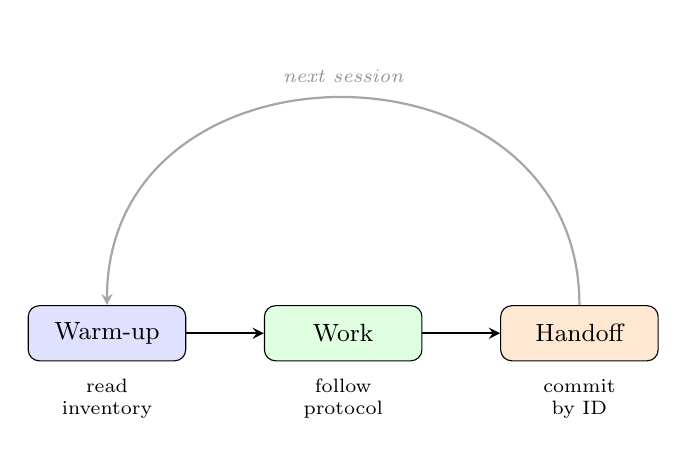
\begin{tikzpicture}[
    phase/.style={draw,rounded corners,minimum width=2.0cm,minimum height=0.7cm,font=\small},
    arrow/.style={->,>=stealth,thick},
]
\node[phase,fill=blue!12]   (warm) at (0,0.6) {Warm-up};
\node[phase,fill=green!12]  (work) at (3,0.6) {Work};
\node[phase,fill=orange!18] (hand) at (6,0.6) {Handoff};
\draw[arrow] (warm) -- (work);
\draw[arrow] (work) -- (hand);
% Loop back ABOVE the boxes (out=90,in=90) so it doesn't cross the descriptors below
\draw[arrow,gray!70,thick]
  (hand.north) to[out=90,in=90,looseness=1.5]
  node[above=2pt,font=\scriptsize\itshape,gray!85] {next session}
  (warm.north);
% Descriptors below each phase
\node[font=\scriptsize,below=0.1cm of warm,align=center] {read\\inventory};
\node[font=\scriptsize,below=0.1cm of work,align=center] {follow\\protocol};
\node[font=\scriptsize,below=0.1cm of hand,align=center] {commit\\by ID};
\end{tikzpicture}
\caption{Session lifecycle. Every session takes the same warm-up
path, whether the prior session ended cleanly or crashed. The
\emph{next session} loop is the same loop on every restart.}
\label{fig:session}
\end{figure}

\textbf{Warm-up.} Before any productive work in a new session: read
the inventory; read the protocol's TL;DR refresher; read the
artefacts the current task touches; spawn supplementary reads (or
explorer agents) for any unfamiliar dependencies. Five to ten
minutes spent on warm-up substantially reduces the rate of phantom
decisions, reference rot, and decided-versus-considered confusion
later in the session.

\textbf{Work.} Apply the edit protocol (\S4.4) to every change.
Cite artefacts by stable identifier in conversation, not by
paraphrase. Use task-tracking primitives to make multi-artefact
edits explicit and atomic. When in doubt about which artefact owns
a fact, stop and confirm before editing.

\textbf{Handoff.} Before declaring the session done: every edit is
committed; every new \textsc{missing} artefact created has a stub
frontmatter and an inventory row; every decision has its ADR;
every raised question has its OQ; \texttt{last\_reviewed} and
\texttt{version} are current on touched artefacts; the inventory's
priority queue reflects the new state. The next session's warm-up
is the previous session's handoff, read by whoever (or whatever)
is doing the next session.

The protocol applies symmetrically across the human and AI
collaborators. Both read the substrate at session start. Both
update it during work. Both leave it consistent at session end.
The asymmetry --- that the AI agent's session is bounded by its
context window in a way the human's is not --- is precisely what
the discipline is designed to compensate for.

% =====================================================================
\section{Every Layer Has a Language and an Oracle}
\label{sec:oracles}
% =====================================================================

The hierarchy of Figure~\ref{fig:hierarchy} says that layers
exist and that changes propagate between them. This section says
what a layer is \emph{made of}. The claim is that every layer of
the hierarchy should be paired with two things: a
\textbf{representation formalism} --- the language in which that
layer's content is stated --- and an \textbf{oracle} --- the
strongest available mechanism for checking work against that
layer's stated intent.

The motivation is sharpest in the AI setting.
\citet{lahiri2026intent} names the central bottleneck of AI-era
work the \emph{intent gap}: the semantic distance between what the
operator means and what the produced artefact does. Generated
output is plausible by construction, not correct by construction,
and AI widens the gap by producing volume faster than scrutiny can
keep up. Crucially, ``there is no oracle for specification
correctness other than the user'': at the topmost layer, only the
human can say whether the stated intent is the intended intent.
Every layer below that can and should have a mechanical or
semi-mechanical oracle. The discipline's layered substrate is how
the user's scarce oracle capacity is spent where nothing else can
substitute for it, while cheaper oracles police every other layer.

The principle is domain-general. In empirical research, the top
layer's oracle is a pre-registered hypothesis tested against
held-out data; in quantitative modelling, agreement with known
analytical solutions; in regulatory drafting, traceability of
every clause to its source obligation. We instantiate the
principle for software (Table~\ref{tab:oracles}) because software
currently has the most mature oracle stack --- not because the
discipline is about software.

% --- Layer / representation / oracle table ---
\begin{table*}[t]
\centering
\small
\begin{tabular}{p{2.6cm} p{4.2cm} p{4.3cm} p{4.3cm}}
\toprule
\textbf{Layer} & \textbf{Representation formalism} & \textbf{Oracle} & \textbf{Guardrail} \\
\midrule
Business behaviour & executable behavioural contracts (Gherkin scenarios) & acceptance runs against the live system & behavioural lock-in of the incumbent before any replacement work \\
Requirements & structured natural language with stable-ID references & human review of a formal restatement --- the one oracle only the user can be & frozen status; ADR-gated unfreeze \\
Design / contracts & Data Dictionaries, schemas, Decision Records & schema validation; contract tests & SSOT; propagation rules \\
Implementation & typed code & compiler and type checker; property tests; postconditions & syntactic constraints on generation (grammar-constrained decoding) \\
Non-functional envelope & measurable NFR contracts: latency, memory, throughput budgets & runtime instrumentation of the incumbent and the replacement & budget assertions in CI; canary comparison against the incumbent \\
\bottomrule
\end{tabular}
\caption{The software instantiation of layer $\to$ (representation,
oracle, guardrail). Other domains substitute their own columns;
the discipline supplies the pairing, not the particular formalisms.}
\label{tab:oracles}
\end{table*}

\paragraph{Why a tower is sound.} The pairing would be decorative
if changes could not be trusted to cross layers. Abstract
interpretation \citep{cousot1977abstract} gives the
theorem-shaped justification: sound approximation between a
concrete and an abstract domain is a Galois connection, and the
composition of two Galois connections is itself a Galois
connection --- so a tower of abstraction layers preserves
soundness layer-by-layer if each adjacent pair does. This
reframes agent divergence precisely: an agent diverges when it
violates the semantic-preservation obligation between the layer
it was instructed at and the layer it produced. The discipline's
forward and reverse propagation rules (\S4.5) are the operational
form of maintaining those connections.

\paragraph{What guardrails can and cannot do.} At the
implementation layer, grammar-constrained decoding can provably
force generated output into a target grammar
\citep{park2025gcd}. The guarantee is syntactic only ---
constraint is not correctness, and it is not even safety: a
benign-looking grammar constraint can itself be used to jailbreak
a model into producing malicious code
\citep{zhang2026gcdjailbreak}. Verification-aware pipelines go
further --- Dafny as a hidden intermediate language compiles
verified code to the target language \citep{li2025dafny}, and
LLM-generated formal postconditions have caught dozens of real
historical bugs while remaining far from complete coverage
\citep{endres2024postconditions}. The stack is real but young,
and it enforces nothing above the layer it operates on. This is
the argument for layered oracles rather than any single
mechanism: each layer's guardrail is blind to the layers above
it.

\paragraph{The residual gap.} One structural fact must be stated
before observability can be read honestly. The operator's
information-processing capacity is finite and the amplifier's
output rate is not matched to it, so the fraction of generated
work that can receive human-level verification falls as the
coupling speeds up; mechanical oracles recover only what can be
formalised; some residue always escapes both. The gap cannot be
closed from inside the loop --- verifying the amplifier's output
with the capacity the amplifier has already saturated is
M\"unchhausen's escape, the system pulling itself out of the
swamp by its own hair. And the gap has a quieter half on the
human side of the centroid: an ever-growing share of the
operator's own model of the work consists of the agent's
renderings, trusted but never checked. \citet{bainbridge1983}
named this shape four decades before the present tooling: the
supervisor of a fast automated process is structurally the
worst-placed participant to catch its errors, while the hands-on
capacity that would catch them atrophies from disuse. The human
mass of Figure~\ref{fig:centroid} drifts too --- not by amnesia
but by induced reliance --- which is why the
decided-versus-considered distinction and the append-only record
exist as much for the operator as for the agent. Faced with the
gap, exactly two postures are coherent: throttle the coupling to
the pace of human verification, surrendering the speed that
justified it; or accept residual error as a design input and
move the human's work up a level --- from verifying outputs to
designing the error-processing architecture itself: boundaries,
invariants, escalation thresholds, and the reversibility that
makes an error caught late cheap rather than fatal. The second
posture is not resignation; it is the law of requisite variety
\citep{ashby1956cybernetics} applied: a controller with less
variety than the system it steers controls through aggregation
and hierarchy, never item by item. This is why the governor of
Figure~\ref{fig:loop} designs guardrails and budgets but does
not sit in the loop as its sensor, and why the accounting later
in this section carries unverified volume as priced debt rather
than counting it as output: the discipline does not close the
residual gap. It contains it, prices it, and escalates what
crosses it.

Out of the sensor path, however, is not out of the room. What
the posture forbids is making the loop's closure depend on the
operator reading everything --- that is the throttle by another
name. It does not forbid watching. The operator retains a
distinct and cheap observational act: sampling the live
trajectory. A reasoning trace is itself an observability
channel, a compressed projection far shorter than the output it
generates, and a wrong turn is visible there earlier than in any
artefact it produces; skimming the trace and interrupting while
the excursion is still small is aggregation-level control in
exactly Ashby's sense, and it is the cheapest correction the
loop admits --- the supervisor's hand on the cord, not the
inspector's eye on every part. The discipline asks only that
this watching stay discretionary: a loop that is safe only while
the human watches has not designed for the residual gap; it has
papered over it with attention.

% --- F10 Observability control loop (two panels, full width) ---
\begin{figure*}[t]
\centering
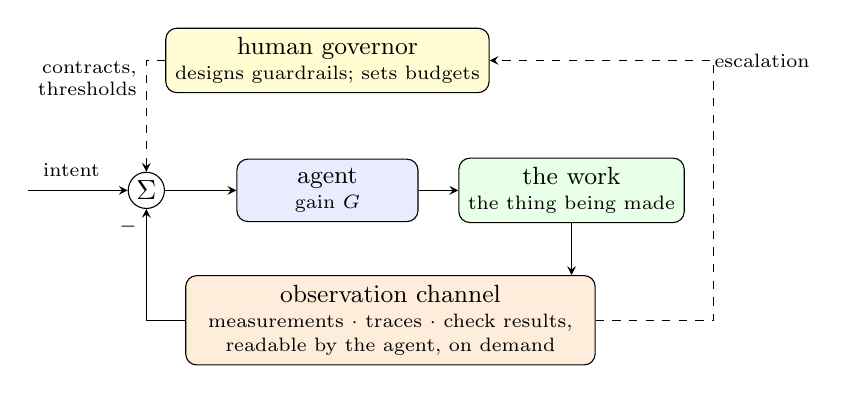
\begin{tikzpicture}[
  blk/.style={draw,rounded corners,minimum height=0.66cm,font=\small,align=center},
  sig/.style={->,>=stealth},
]
% comparator
\node[draw,circle,minimum size=0.46cm,inner sep=0pt] (cmp) at (0,0) {$\Sigma$};
\draw[sig] (-1.5,0) -- (cmp);
\node[font=\scriptsize,anchor=south] at (-0.95,0.05) {intent};
% forward path
\node[blk,fill=blue!8,minimum width=2.3cm]  (agent) at (2.3,0) {agent\\[-2pt]\scriptsize gain $G$};
\node[blk,fill=green!9,minimum width=2.4cm] (work)  at (5.4,0)
  {the work\\[-2pt]\scriptsize the thing being made};
\draw[sig] (cmp) -- (agent);
\draw[sig] (agent) -- (work);
% feedback path
\node[blk,fill=orange!14,minimum width=5.2cm] (obs) at (3.1,-1.65)
  {observation channel\\[-2pt]\scriptsize measurements $\cdot$ traces $\cdot$ check results,\\[-2pt]\scriptsize readable by the agent, on demand};
\draw[sig] (work.south) -- (obs.north -| work.south);
\draw[sig] (obs.west) -| (cmp.south)
  node[pos=0.92,left,font=\scriptsize] {$-$};
% human governor
\node[blk,fill=yellow!18,minimum width=3.9cm] (human) at (2.3,1.65)
  {human governor\\[-2pt]\scriptsize designs guardrails; sets budgets};
\draw[sig,dashed] (human.west) -| (cmp.north)
  node[pos=0.58,left,font=\scriptsize,align=right] {contracts,\\thresholds};
\draw[sig,dashed] (obs.east) -- ++(1.5,0) |- (human.east)
  node[pos=0.52,right,font=\scriptsize,align=left] {escalation};
\end{tikzpicture}
\hspace{0.55cm}
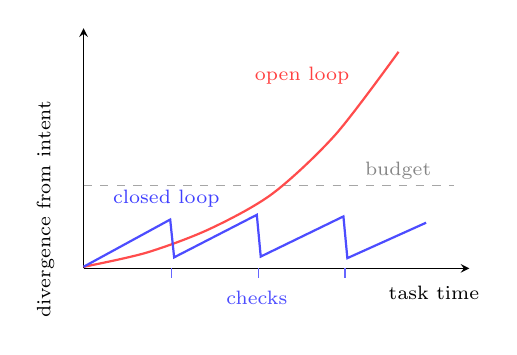
\begin{tikzpicture}
% axes
\draw[->,>=stealth] (0,0) -- (4.9,0);
\node[font=\scriptsize,anchor=north] at (4.45,-0.1) {task time};
\draw[->,>=stealth] (0,0) -- (0,3.05);
\node[font=\scriptsize,anchor=south,rotate=90] at (-0.25,0.75) {divergence from intent};
% budget line
\draw[dashed,gray!70] (0,1.05) -- (4.7,1.05);
\node[font=\scriptsize,gray!95,anchor=west] at (3.45,1.24) {budget};
% open loop
\draw[red!70,thick] plot[smooth] coordinates
  {(0,0.02) (0.8,0.2) (1.6,0.5) (2.4,0.95) (3.2,1.7) (4.0,2.75)};
\node[font=\scriptsize,red!75,anchor=east] at (3.5,2.45) {open loop};
% closed loop sawtooth
\draw[blue!70,thick] (0,0.02) -- (1.1,0.62) -- (1.15,0.14)
  -- (2.2,0.68) -- (2.25,0.15) -- (3.3,0.66) -- (3.35,0.13)
  -- (4.35,0.58);
\node[font=\scriptsize,blue!75,anchor=west] at (0.25,0.88) {closed loop};
% check marks
\foreach \x in {1.12,2.22,3.32} \draw[blue!60] (\x,0) -- (\x,-0.12);
\node[font=\scriptsize,blue!70,anchor=north] at (2.2,-0.16) {checks};
\end{tikzpicture}
\caption{Observability closes the loop. \emph{Left:} the coupling
as a control loop. The human governor designs the guardrails ---
contracts, budgets, escalation thresholds --- but does not sit in
the loop as its sensor; the agent is the forward-path gain; the
work's state feeds back through an observability channel the
agent can query directly. \emph{Right:} the consequence.
Amplification is indifferent to sign: run open-loop, the gain
that compounds progress compounds divergence at the same rate;
run closed-loop, each check detects the excursion while it is
small, and correction stays cheap.}
\label{fig:loop}
\end{figure*}

\paragraph{Observability closes the loop.} An oracle the agent
cannot query is not a guardrail; it is an audit. For guardrails
to be enforced \emph{in the loop} --- during the work, not after
it --- the state of the work must be observable \emph{to the
agent}: measurements, traces, and check results exposed as
channels the agent can consult cheaply, repeatedly, and without
human mediation (Figure~\ref{fig:loop}, left). In the software
instantiation these are logs, telemetry, and oracle runs behind
queryable service endpoints and tool interfaces; in research,
analysis outputs and their provenance; in a physical design,
simulation and measurement results. The form varies; the
requirement --- that the thing being made can be interrogated
about its actual state, by the agent, at any moment --- does not.
The reason is the amplifier structure of the coupling. An
agent is gain: it multiplies operator intent into volume. But
gain is indifferent to sign --- the same amplification that
compounds progress compounds divergence --- and an amplifier run
open-loop diverges at the rate of its gain
(Figure~\ref{fig:loop}, right). We suggest this is the mechanism
behind the slowdown regime of \S2: couplings that turn
net-negative not because the model is weak, but because generated
volume runs unobserved long enough that correcting the divergence
costs more than the generation saved. A closed loop inverts the
economics: each check detects excursion while it is small, so the
cost of correction stays proportional to the excursion rather
than to the volume built on top of it --- in centroid terms,
observability is what makes reversion cheap. And the loop
compounds across sessions through the substrate: what each check
finds --- violations, escalations, the decisions they forced ---
is deposited as substrate records, so the fast within-session
loop feeds the slow across-session loop that the substrate
carries (Figure~\ref{fig:system}). The human's place in
this loop is not sensor but \emph{designer}: choosing the
contracts and budgets of Table~\ref{tab:oracles}, the thresholds
at which the agent must stop and escalate, and the cadence of
checks. Efficient coupling is a control-design problem. Give the
operator controls that cap excursion early, and the amplifier
works for you; omit them, and it works against you --- at the
same gain.

\paragraph{The non-functional envelope.} The formal literature on
constraining AI-generated work is overwhelmingly about functional
correctness; the non-functional envelope --- latency, memory,
throughput, operational cost --- is nearly absent from it. Yet in
brownfield work the envelope is often the binding constraint, and
it admits an oracle most projects already own: \emph{the incumbent
system}. Before replacing a latency-sensitive process, capture its
observable behaviour as executable contracts \emph{and} its
runtime profile as measured budgets --- on a JVM, allocation and
memory behaviour are recoverable from JMX-level statistics, or at
finer resolution by bytecode-level instrumentation of allocation
sites --- and hold the replacement to those budgets continuously.
The incumbent becomes the oracle at every layer it can speak for.
\S\ref{sec:example} shows this in flight. Evidence on
LLM-generated behavioural specifications points the same way:
quality ratings are high, but omissions and hallucinations occur
at rates that require systematic human review
\citep{hassani2025gherkin} --- which is exactly the layered
posture: the mechanical oracle runs everywhere it can, and the
human oracle reviews where only the human can.

% --- F12 Substrate as compressed source ---
\begin{figure}[t]
\centering
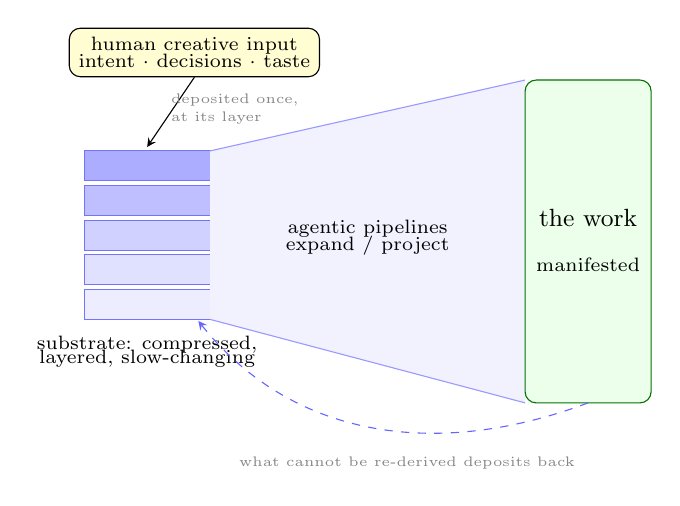
\begin{tikzpicture}[sig/.style={->,>=stealth}]
% human creative input
\node[draw,rounded corners,fill=yellow!18,font=\scriptsize,align=center]
  (crea) at (-2.0,2.35) {human creative input\\[-2pt]intent $\cdot$ decisions $\cdot$ taste};
\draw[sig] (crea.south) -- (-2.6,1.15);
\node[font=\tiny,gray!95,anchor=west] at (-2.42,1.74) {deposited once,};
\node[font=\tiny,gray!95,anchor=west] at (-2.42,1.52) {at its layer};
% substrate strata
\foreach \i/\c in {0/blue!32,1/blue!25,2/blue!18,3/blue!12,4/blue!7}
  \draw[fill=\c,draw=blue!55]
    (-3.4,1.1-\i*0.44) rectangle (-1.8,1.1-\i*0.44-0.38);
\node[font=\scriptsize,align=center] at (-2.6,-1.45)
  {substrate: compressed,\\[-3pt]layered, slow-changing};
% expansion cone
\fill[blue!5] (-1.8,1.1) -- (2.2,2.0) -- (2.2,-2.1) -- (-1.8,-1.04) -- cycle;
\draw[blue!40] (-1.8,1.1) -- (2.2,2.0);
\draw[blue!40] (-1.8,-1.04) -- (2.2,-2.1);
\node[font=\scriptsize,align=center] at (0.2,0.0)
  {agentic pipelines\\[-2pt]expand $/$ project};
% the work
\draw[fill=green!8,draw=green!45!black,rounded corners]
  (2.2,-2.1) rectangle (3.8,2.0);
\node[font=\small,align=center] at (3.0,0.25) {the work};
\node[font=\scriptsize,align=center] at (3.0,-0.35) {manifested};
% return of new decisions
\draw[sig,dashed,blue!60] (3.0,-2.1)
  .. controls (1.0,-2.85) and (-0.8,-2.5) .. (-1.95,-1.06);
\node[font=\tiny,gray!95,anchor=north] at (0.7,-2.66)
  {what cannot be re-derived deposits back};
\end{tikzpicture}
\caption{The substrate as compressed source. The strata are the
hierarchy of Figure~\ref{fig:hierarchy}: shortest description on
top, derivable detail beneath. The human deposits only what no
pipeline can re-derive --- intent, decisions, taste --- once, at
the layer where it belongs; agentic pipelines expand the
compressed representation into the manifested work, with the
oracles of Table~\ref{tab:oracles} bounding the distortion of the
expansion (Figure~\ref{fig:loop}); discoveries that cannot be
re-derived deposit back. Everything else is cognitive load ---
exactly what the human no longer carries.}
\label{fig:projection}
\end{figure}

\paragraph{The substrate as compressed source.} There is a
reading of the whole apparatus in one information-theoretic
sentence: the substrate is a \emph{compressed representation of
the work being manifested}, and the agentic pipeline is its
decompressor (Figure~\ref{fig:projection}). The hierarchy of
layers makes the compression progressive: the top layer is the
shortest description, and each layer beneath expands it with
detail that is --- crucially --- \emph{derivable}, given the
layers above and the facts on record. What must actually be
stored is what no pipeline can re-derive: the choices among
alternatives, the intent behind them, the taste that selected
this design over that one. It is no accident that the append-only
Decision Records are the substrate's most protected artefacts;
they are the incompressible kernel. The reading has a standard
formalisation. In algorithmic information theory, the information
in a deposit $x$ that is derivable from a substrate $S$ is
captured by conditional complexity $K(x \mid S)$ --- the length
of the shortest program producing $x$ given $S$ as input
\citep{kolmogorov1965, li2008kolmogorov}. Relative to a pipeline
$d$, a contribution is \emph{derivable} exactly when
$K_d(x \mid S)$ is negligible, and the creative kernel of a
deposit is its conditional description length given the prior
substrate and the pipeline. The pipeline-relativity is a feature,
not a defect: as pipelines strengthen, more becomes derivable and
the kernel shrinks --- the formal shadow of the operator's
migration up the abstraction hierarchy. This gives the discipline's
purpose its sharpest statement: the entire apparatus exists to
\textbf{separate genuine human creative input from cognitive
load}. The human supplies the bits that cannot come from anywhere
else --- once, at the layer where they belong; everything
derivable --- the expansion, the bookkeeping, the propagation,
the re-derivation that flat collaboration forces the human to
repeat every session --- is carried by the substrate and executed
by the pipeline, with the oracles bounding the distortion of the
expansion. The failure modes of \S2 read naturally in this frame:
drift is decoder error accumulating unchecked; a phantom decision
is the decoder inventing source bits; restart cost is
retransmission of content that should have been stored
compressed.

\paragraph{What productivity means here.} The contested record of
\S2 is partly a dispute about the measurand. Classical
productivity --- output volume per unit time --- was a serviceable
proxy while production was the scarce step. In a coupled
environment it fails twice over: volume is precisely what the
amplifier inflates, and it inflates divergence as willingly as
progress; and perceived productivity tracks volume, which is why
developers in the measured slowdown regime sincerely felt
faster. The frames of this section supply the replacement. The
scarce inputs of a coupling are three: the human's creative kernel
(the non-derivable bits), the human's oracle capacity (review and
approval where no mechanical oracle can substitute), and the
calendar time of the loop. The genuine output is not generated
volume but \emph{validated intent made durable}: expansions that
survived their layer's oracle, and the residue of the session ---
decisions recorded, questions resolved, maps updated --- deposited
into the substrate so that it is never paid for twice.
Productivity, in the environment this paper proposes, is the rate
at which durable, validated intent accumulates per unit of scarce
human input. Generated volume drops out of the measure entirely;
on the trajectory scale, unverified volume is not output at all
--- it is rework not yet scheduled.

\paragraph{From definition to measurement.} $K$ is uncomputable,
but the definition admits computable surrogates --- and the
discipline is self-instrumenting: every term of the measure
corresponds to an event stream the substrate already
externalises. Kernel content is estimable by
minimum-description-length surrogates \citep{rissanen1978} or,
directly practicable today, by the code length a strong language
model assigns to a deposit conditioned on the prior substrate,
$-\log p(x \mid S)$ --- language models are, formally,
general-purpose compressors \citep{deletang2023lmic} --- so
derivable content scores near zero while a direction-changing
decision scores high. Validation weight is the locked contracts'
\emph{discriminating power}: the fraction of injected behavioural
mutations they catch \citep{endres2024postconditions}, which
resists inflation by padding in a way raw contract counts do not.
Durability is survival: the fraction of deposited artefacts still
referenced and un-invalidated $k$ sessions later, together with
the warm-up cost curve, which stays flat under working durability
and grows with project size without it. The denominator is logged
by construction --- kernel time, oracle time (approvals at L2 are
events), load time. Unverified volume outstanding is the
liability account, and churn attributable to failed oracles is
the debt coming due. Assembled, the accounting is compact.
Writing $S$ for the substrate before deposit $x$ and $d$ for the
pipeline,
\[
\kappa(x) \;=\; K(x \mid S, d) \;\approx\; -\log p_{\theta}(x \mid S)
\]
is the deposit's kernel content --- its conditional description
length, estimated by a strong model's code length. Over the
deposits $\mathcal{D}_T$ of a period,
\[
I_T \;=\; \sum_{x \in \mathcal{D}_T} \kappa(x)\, v(x)\, s_k(x)
\]
is validated intent made durable, with $v(x) \in [0,1]$ the
mutation kill rate of the contracts locked by $x$ and
$s_k(x)$ its survival $k$ sessions on. Then
\[
P_T \;=\; \frac{I_T \;-\; \lambda\, \Delta D_T}
               {t_{\mathrm{kernel}} + t_{\mathrm{oracle}} + t_{\mathrm{load}}}
\]
is productivity: net accrual per unit of scarce human time, where
$\Delta D_T$ is the change in divergence debt --- unverified
volume priced at its empirically observed rework rate --- and
$\lambda$ its weight. Note what $P_T$ does not contain: gross
generated volume $V_T$, the quantity felt productivity tracks.
The ratio $V_T / I_T$ is a project's calibration failure,
measurable continuously instead of discovered in a randomised
trial. None of this needs apparatus beyond
\S\ref{sec:governance}: the metering layer is the L1 integrity
watchdog, read for a second purpose.

\paragraph{A research horizon, flagged as such.} The pairing in
Table~\ref{tab:oracles} is stated, not derived, and the
estimators above are surrogates, not theory. A formal treatment
would model the human--agent channel in rate--distortion terms ---
rate as specification effort, distortion as residual intent
misalignment --- for which program-induction work already supplies
a skeleton \citep{zhou2024ratedistortion}, with
\citet{felleisen1991expressive}'s expressiveness giving the
complementary inter-layer measure. On that view, the optimal
granularity of a layer's representation is not fixed: it moves
with the ability of the team operating the coupling. We flag this
deliberately and do not develop it here; the discipline stands on
the weaker, practicable claim that \emph{some} explicit pairing at
every layer beats an implicit one at any.

% =====================================================================
\section{Human Governance, Agent Execution}
\label{sec:governance}
% =====================================================================

The discipline's \emph{content} --- six artefact categories,
stable identifiers, the status lifecycle, the edit protocol,
propagation rules, anti-patterns --- is fixed by
\S\ref{sec:discipline}. Its \emph{execution model} is not. As
specified, every step is performed by the operator; left
there, the discipline would carry a manual burden that does not
scale with project complexity, and would invite the objection
that autonomous memory systems will make it obsolete. The
convergence documented in \S3.3 argues the opposite posture:
Shared Substrate is the \textbf{human-governance schema} over
substrate execution, agnostic to who --- or what --- performs the
execution.

% --- F9 Adoption stack ---
\begin{figure}[t]
\centering
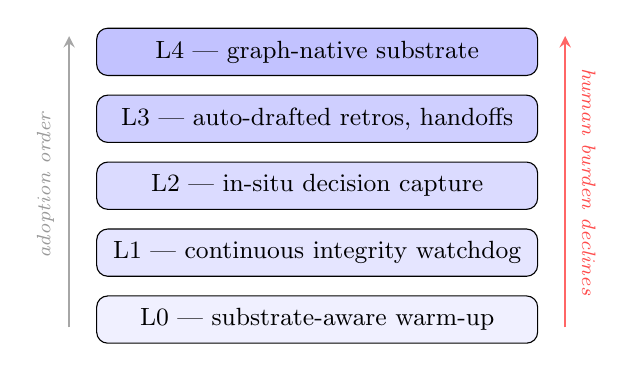
\begin{tikzpicture}[
    lyr/.style={draw,rounded corners,minimum width=5.6cm,minimum height=0.6cm,font=\small,anchor=center},
]
\node[lyr,fill=blue!6]  (l0) at (0,0)    {L0 --- substrate-aware warm-up};
\node[lyr,fill=blue!10] (l1) at (0,0.85) {L1 --- continuous integrity watchdog};
\node[lyr,fill=blue!14] (l2) at (0,1.70) {L2 --- in-situ decision capture};
\node[lyr,fill=blue!19] (l3) at (0,2.55) {L3 --- auto-drafted retros, handoffs};
\node[lyr,fill=blue!24] (l4) at (0,3.40) {L4 --- graph-native substrate};
\draw[->,>=stealth,thick,gray!70] (-3.15,-0.1) -- (-3.15,3.6);
\node[rotate=90,font=\scriptsize\itshape,gray!80] at (-3.45,1.7) {adoption order};
\draw[->,>=stealth,thick,red!60] (3.15,-0.1) -- (3.15,3.6);
\node[rotate=-90,font=\scriptsize\itshape,red!70] at (3.45,1.75) {human burden declines};
\end{tikzpicture}
\caption{The adoption stack. Each layer delegates more substrate
execution to agents; the discipline's semantics are unchanged at
every layer. L0 and L1 adopt first; L4 is the discipline's mature
form. The human's residual surface --- intent, decision approval,
scope, voice --- does not delegate.}
\label{fig:stack}
\end{figure}

The delegation is codified as a five-layer adoption stack
(Figure~\ref{fig:stack}).

\textbf{L0 --- substrate-aware warm-up.} The session warm-up of
\S4.7, performed by the agent instead of the human. The static
baseline costs nothing: modern agent harnesses auto-load a small
project-root instruction file at session start, and that file ---
versioned, edit-protocol-governed, a \emph{pointer} to the
canonical artefacts and never a restatement of them --- turns the
harness's existing behaviour into the warm-up entry point. The
pattern is agent-agnostic in semantics and platform-specific only
in filename; the discipline commits to the pattern, not to any
vendor's loader. The dynamic form is richer: an agent that walks
the \texttt{depends\_on} closure of the current task and reads
what it finds.

\textbf{L1 --- continuous integrity watchdog.} Background checks
that need no judgement: every cross-reference resolves to an
artefact whose frontmatter \texttt{id} matches; every file has an
inventory row and every row a file; frontmatter schemas validate;
\textsc{stable} artefacts unreviewed at a milestone freeze
auto-degrade to \textsc{stale}; orphans and cycles are flagged.
None of this is novel tooling --- linters, schema validators,
graph checks --- and none of it requires judgement, which is
exactly why it delegates first. L1 is the substrate's own
observability channel: the closed loop of \S\ref{sec:oracles}
pointed at the artefact graph itself.

\textbf{L2 --- in-situ decision capture.} The agent drafts the ADR
at the moment a decision is made in conversation, rather than
relying on the human to remember to write it afterwards. The
human approves before the draft becomes a record: an unapproved
auto-drafted ADR is not a decision, it is a phantom decision with
better formatting. L2 targets the single most consequential
failure mode (\S2.4) at its source.

\textbf{L3 --- auto-drafted retrospectives and handoffs.} Session
summaries, next-session prompts, and the inventory's priority
queue populated from observable state --- commits, artefact
touches, resolved and raised questions --- with the human editing
rather than authoring.

\textbf{L4 --- graph-native substrate.} The artefact graph held as
a first-class knowledge graph, with the markdown artefacts as
rendered views and the atlas of Figure~\ref{fig:atlas} drawn by
tooling rather than by hand.

Adoption order matters: L0 and L1 first --- low cost, immediate
utility, independent of each other; L2 and L3 only after L0/L1
have proven reliable, because they draft content in the human's
voice; L4 is the discipline's mature form, not its entry point.
At every layer the human's residual surface is the same:
\textbf{intent declaration, decision approval, scope governance,
and voice authority over substantive prose.} That surface does
not delegate --- it is what governance means. The stack changes
who executes the discipline; accountability for the substrate,
like authorship of the project, stays with the person. Seen
through the compression reading of \S\ref{sec:oracles}, the stack
is a distillation apparatus: layer by layer it strips cognitive
load away from the person until what remains is only the input no
pipeline can generate --- the creative kernel. Delegation is not
the human doing less; it is the human's effort converging on the
only work that was ever irreducibly theirs.

% --- F11 The coupled system in action (panorama, full width) ---
\begin{figure*}[t]
\centering
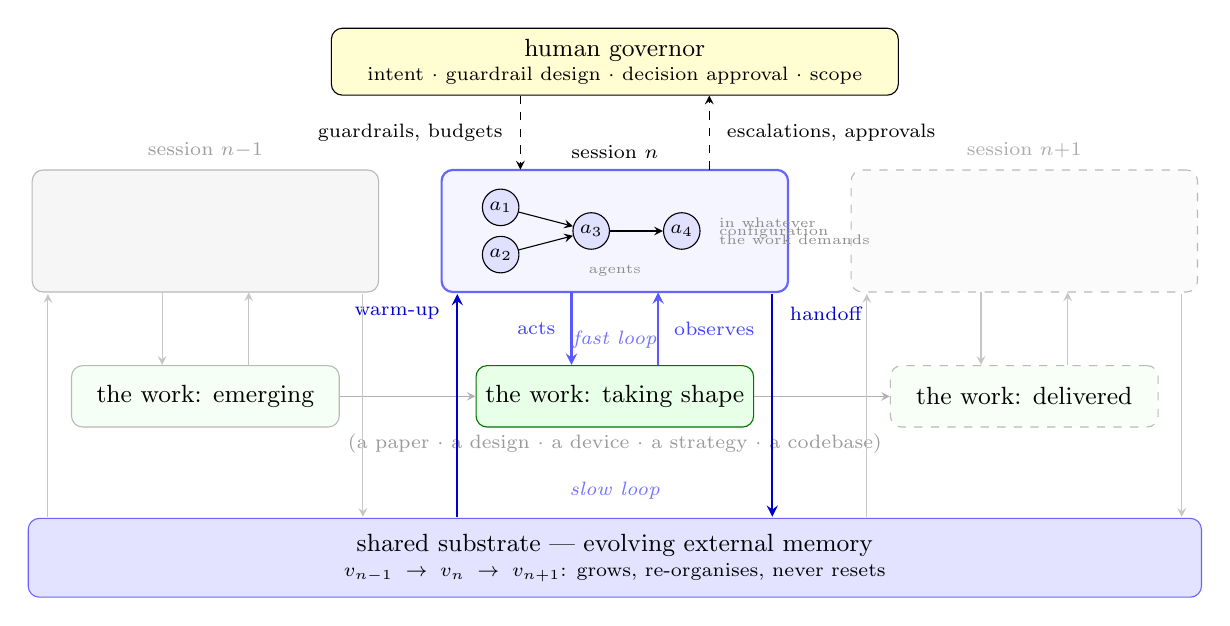
\begin{tikzpicture}[
  sess/.style={draw,rounded corners,minimum width=4.4cm,minimum height=1.55cm},
  wrk/.style={draw,rounded corners,minimum width=3.4cm,minimum height=0.78cm,font=\small,align=center},
  ag/.style={draw,circle,inner sep=1.5pt,font=\scriptsize,fill=blue!12},
  sig/.style={->,>=stealth},
  fade/.style={->,>=stealth,gray!45,thin},
]
% ---------- human governor ----------
\node[draw,rounded corners,fill=yellow!18,minimum width=7.2cm,minimum height=0.85cm,font=\small,align=center]
  (gov) at (0,5.15)
  {human governor\\[-2pt]\scriptsize intent $\cdot$ guardrail design $\cdot$ decision approval $\cdot$ scope};
% ---------- session row ----------
\node[sess,draw=gray!55,fill=gray!7]        (sm) at (-5.2,3.0) {};
\node[font=\scriptsize,gray!75,anchor=south] at (-5.2,3.80) {session $n{-}1$};
\node[sess,draw=blue!60,fill=blue!4,thick]  (sn) at (0,3.0) {};
\node[font=\scriptsize,anchor=south] at (0,3.80) {session $n$};
\node[sess,draw=gray!55,dashed,fill=gray!3] (sp) at (5.2,3.0) {};
\node[font=\scriptsize,gray!65,anchor=south] at (5.2,3.80) {session $n{+}1$};
% agents inside main session: two parallel feeding an integrator, then a checker
\node[ag] (a1) at (-1.45,3.30) {$a_1$};
\node[ag] (a2) at (-1.45,2.70) {$a_2$};
\node[ag] (a3) at (-0.30,3.00) {$a_3$};
\node[ag] (a4) at (0.85,3.00) {$a_4$};
\draw[sig] (a1) -- (a3);
\draw[sig] (a2) -- (a3);
\draw[sig] (a3) -- (a4);
\node[font=\tiny,gray!90,anchor=west,align=left] at (1.20,3.00)
  {in whatever\\[-3pt]configuration\\[-3pt]the work demands};
\node[font=\tiny,gray!90,anchor=south] at (0,2.30) {agents};
% ---------- work row ----------
\node[wrk,draw=gray!55,fill=green!4]          (wm) at (-5.2,0.9) {the work: emerging};
\node[wrk,draw=green!45!black,fill=green!9]   (wn) at (0,0.9) {the work: taking shape};
\node[wrk,draw=gray!55,dashed,fill=green!3]   (wp) at (5.2,0.9) {the work: delivered};
\draw[sig,gray!60] (wm) -- (wn);
\draw[sig,gray!60] (wn) -- (wp);
\node[font=\scriptsize,gray!80] at (0,0.30)
  {(a paper $\cdot$ a design $\cdot$ a device $\cdot$ a strategy $\cdot$ a codebase)};
% fast loop (main session): act / observe
\draw[sig,blue!65,thick] (-0.55,2.22) -- (-0.55,1.30);
\node[font=\scriptsize,blue!75,anchor=east] at (-0.63,1.76) {acts};
\draw[sig,blue!65,thick] (0.55,1.30) -- (0.55,2.22);
\node[font=\scriptsize,blue!75,anchor=west] at (0.63,1.76) {observes};
\node[font=\scriptsize\itshape,blue!55] at (0,1.62) {fast loop};
% fast loops (ghost sessions)
\draw[fade] (-5.75,2.22) -- (-5.75,1.30);
\draw[fade] (-4.65,1.30) -- (-4.65,2.22);
\draw[fade] (4.65,2.22) -- (4.65,1.30);
\draw[fade] (5.75,1.30) -- (5.75,2.22);
% ---------- substrate band ----------
\node[draw=blue!60,rounded corners,fill=blue!11,minimum width=14.9cm,minimum height=1.0cm,font=\small,align=center]
  (sub) at (0,-1.15)
  {shared substrate --- evolving external memory\\[-2pt]
   \scriptsize $v_{n-1}\;\rightarrow\;v_{n}\;\rightarrow\;v_{n+1}$:
   grows, re-organises, never resets};
% slow loop (main session): warm-up / handoff
\draw[sig,blue!80!black,thick] (-2.0,-0.63) -- (-2.0,2.20);
\node[font=\scriptsize,blue!80!black,anchor=east] at (-2.10,1.95) {warm-up};
\draw[sig,blue!80!black,thick] (2.0,2.20) -- (2.0,-0.63);
\node[font=\scriptsize,blue!80!black,anchor=west] at (2.10,1.95) {handoff};
\node[font=\scriptsize\itshape,blue!55] at (0,-0.30) {slow loop};
% slow loops (ghost sessions)
\draw[fade] (-7.2,-0.63) -- (-7.2,2.20);
\draw[fade] (-3.2,2.20) -- (-3.2,-0.63);
\draw[fade] (3.2,-0.63) -- (3.2,2.20);
\draw[fade] (7.2,2.20) -- (7.2,-0.63);
% ---------- governance wires ----------
\draw[sig,dashed] (-1.2,4.72) -- (-1.2,3.78);
\node[font=\scriptsize,anchor=east] at (-1.30,4.25) {guardrails, budgets};
\draw[sig,dashed] (1.2,3.78) -- (1.2,4.72);
\node[font=\scriptsize,anchor=west] at (1.30,4.25) {escalations, approvals};
\end{tikzpicture}
\caption{The coupled system in action, in no domain's vocabulary.
The human governs; agents --- in whatever configuration the work
demands --- act within a session; the thing being made advances
left to right. Two nested feedback loops drive it: the
\emph{fast loop} within a session (agents act on the work and
observe its actual state against the guardrails,
\S\ref{sec:oracles}), and the \emph{slow loop} across sessions
(warm-up reverts to the substrate, handoff deposits back, \S4.7).
Sessions end and agents are swapped; the evolving substrate never
resets --- it carries the coupling's accumulated understanding
forward.}
\label{fig:system}
\end{figure*}

Figure~\ref{fig:system} assembles the whole coupled system in one
picture, deliberately free of any domain's vocabulary. Read it as
the paper in miniature. The work being manifested --- a paper, a
design, a device, a strategy, a codebase --- advances under two
nested loops. The fast loop is \S\ref{sec:oracles}: within a
session, agents act on the work and observe its actual state
against the layer contracts. The slow loop is \S4.7: across
sessions, every participant reverts to the substrate at warm-up
and deposits back at handoff --- and what the fast loop finds,
the slow loop keeps, because violations, escalations, and the
decisions they force are themselves deposited as substrate
records. The human sits above both loops, governing; the
substrate sits beneath both, evolving. It is the only element in
the picture that neither resets nor retires: agents are swapped,
sessions end, the work ships --- the evolving external memory
carries the coupling's accumulated understanding forward into
whatever comes next.

% =====================================================================
\section{The Synthesis: Discipline $\leftrightarrow$ Cognitive Principle $\leftrightarrow$ Failure Mode}
\label{sec:synthesis}
% =====================================================================

This section is the paper's central synthesis. Each element of
Shared Substrate from \S\ref{sec:discipline} maps to a
cognitive principle from \S\ref{sec:foundations} that grounds it,
to a failure mode from \S\ref{sec:failures} that it mitigates, and
to the adoption-stack layer (\S\ref{sec:governance}) that can
execute it on the operator's behalf.
Table~\ref{tab:synthesis} lays out the mapping.

% --- F6 Mapping Synthesis (table, full-width) ---
\begin{table*}[t]
\centering
\small
\begin{tabular}{p{3.5cm} p{4.9cm} p{4.2cm} p{1.9cm}}
\toprule
\textbf{Discipline element} & \textbf{Cognitive principle} & \textbf{Failure mode addressed} & \textbf{Executed by} \\
\midrule
Hierarchy of abstraction layers & Marr's three levels of analysis \citep{marr1982vision}; hierarchical predictive coding \citep{clark2013whatever} & Drift across iterations; lost intent & human; L4 \\
Single Source of Truth + DRY-for-prose & External representations \citep{scaife1996external}; cognitive load \citep{sweller1988cognitive} & Decided-vs-considered confusion; reference rot & L1 \\
Stable identifiers (KB-N, ADR-N, OQ-N) & Boundary objects \citep{star1989boundary}; persistent symbolic anchors & Reference rot; phantom decisions & L1 \\
Append-only Decision Records & Distributed cognition \citep{hutchins1995}; preservation of reasoning trail & Phantom decisions; silent reversal & L2 + human approval \\
Status lifecycle (MISSING $\to$ DRAFT $\to$ STABLE $\to$ STALE) & Schema theory \citep{bartlett1932remembering}; affordances of state & Drift; stale knowledge & L1 \\
Edit protocol with trivial-fix lane & Cognitive load theory \citep{sweller1988cognitive}; chunking \citep{miller1956magical, cowan2001magical} & Restart cost; over-ceremony abandonment & L1--L3 \\
Glossary as authoritative semantic anchor & Encoding specificity \citep{tulving1973encoding} & Terminology drift & L1 \\
Session warm-up + handoff protocol & Cognitive offloading \citep{risko2016offloading} & Restart cost; context-window saturation & L0, L3 \\
\bottomrule
\end{tabular}
\caption{The synthesis. Each discipline element, the cognitive
principle that grounds it, the failure mode (\S\ref{sec:failures})
it addresses, and the adoption-stack layer (\S\ref{sec:governance})
that can execute it. ``Human'' marks work that does not delegate.}
\label{tab:synthesis}
\end{table*}

The shape of the table matters as much as its content. Every
discipline element has a cognitive precedent, and every discipline
element addresses an observable failure. The discipline is not
arbitrary, and it is not a list of best practices. It is a small
set of structural choices, each with two sources of justification:
why it should work (the cognitive principle) and what happens when
it is absent (the failure mode).

Three readings of the table are useful. From left to right, it
answers ``why these elements?''. From right to left, it answers
``what to use against this failure?''. Down the final column, it
answers ``what must I still do myself?'' --- and the answer is
short: govern the hierarchy, approve the decisions. The redundancy
is the synthesis's robustness: every element is on the table for
independent reasons.

A reader pressed for time should read \S1 and
Table~\ref{tab:synthesis}. The argument of the paper survives the
reduction.

% =====================================================================
\section{Two Worked Examples}
\label{sec:example}
% =====================================================================

We illustrate Shared Substrate twice: once on a greenfield
multi-month research project, once on a brownfield enterprise
replacement under a hard time-box. In both cases specifics are
generalised, and in both the engineering content is not the point.
The point is the substrate trajectory.

\subsection{Greenfield: a research-to-production bridge}

The first project was a live algorithmic-execution engine bridging
a research backtesting framework to a regulated broker.

The project began as a chat. The author described the
problem: a backtesting framework that produces strategies, a broker
API to send them to live, the gap between the two. The first
artefact deposited to the substrate was a Requirements document ---
flat, around three and a half thousand words, the author's
first pass at what would be built and why.

The second artefact was a Context Inventory, listing the categories
of substrate the project would need: Knowledge Bases, Inventories,
Data Dictionaries, Decision Records, Open Questions, Glossary. The
inventory was at first largely \textsc{missing}; it named the
artefacts that would be needed without yet writing any.

The third artefact was a Context Protocol --- the discipline
document specifying how the substrate would be edited, how
cross-references would work, what the status lifecycle was. The
protocol came before most of the content because it determined how
the content would be added.

From there the substrate grew. The first Knowledge Base captured
the strategy taxonomy --- the archetypes the project would support.
That KB raised ten Open Questions about scope. The author
made decisions on those OQs in a single working session; the
decisions became the project's first set of Architectural Decision
Records. The KB updated to mark the OQs as
\textsc{resolved-by-adr}; the OQs were not deleted, just
re-statused.

Knowledge Bases on the broker's API capabilities and pacing limits
followed. A Cost Dictionary on the project's cost models. A
Companion Projects map clarifying boundaries with related work. A
Frameworks Survey reviewing existing solutions and recording which
were adopted, studied, or rejected --- and why. Within a few
working sessions, thirteen Knowledge Bases existed; three
Inventories; nineteen Architectural Decision Records; twenty-two
Open Questions; one Glossary that had absorbed the terminology
sections of multiple other artefacts.

The Requirements document, originally a flat draft, underwent a
v0.2 pass: sections that had been narrative summaries of survey
content, decision rationale, and open questions were collapsed into
stable-identifier references to the relevant Knowledge Bases,
Architectural Decision Records, and Open Questions. The document
became more authoritative and easier to update --- because the
content it had been carrying now lived in artefacts whose
discipline was to be authoritative.

The substrate trajectory is the point. The project did not begin
with a plan and execute it. It began with the cheapest possible
substrate (a Requirements document) and grew the substrate as the
work demanded it, with the discipline ensuring that every growth
step left the artefact graph coherent. By the time implementation
began, the substrate was sufficient to absorb a session's worth of
work without drift, and the author could resume after a break
of weeks without reconstruction cost.

The metrics --- thirteen KBs, nineteen ADRs, twenty-two OQs ---
are incidental. The trajectory --- substrate as living artefact,
growing to match the project's demand for stability --- is the
substance.

\subsection{Brownfield: replacing a legacy process in a regulated
enterprise}

The second example is brownfield, and adversarial in the way
enterprise work usually is. At a regulated financial institution,
the author replaced a legacy low-latency Java process --- a
component that had accreted responsibilities for years, did too
much, and had become hard to evolve --- with a new implementation
stood up from scratch in roughly two weeks, the second of which
was spent almost entirely inside the non-functional envelope:
allocation behaviour, memory footprint, latency profile.

The trajectory, not the speed, is the point, and it followed the
shape of this paper. The work began not with code but with a
top-down design investigation: recovering what the incumbent
actually did --- as opposed to what its documentation said it did
--- and an explicit phased plan for standing the replacement up
and retiring the incumbent. The incumbent's observable behaviour
was locked in as executable contracts before replacement work
began, so that ``done'' meant \emph{equivalent where equivalence
was intended} rather than \emph{looks right}. The non-functional
envelope was locked the same way (\S\ref{sec:oracles}): the
incumbent's memory and latency profile captured by runtime
instrumentation --- JMX-level statistics first, bytecode-level
allocation capture where finer resolution was needed --- and held
as budgets the replacement had to meet continuously, queryable
in-loop so that a violation surfaced during implementation rather
than at review (Figure~\ref{fig:loop}). Inside those
guardrails, agent-assisted implementation was fast precisely
because it was safe: the incumbent was the oracle at every layer
it could speak for, and each phase of the plan mapped to one
abstraction layer with its own representation and its own oracle.

What the time-box demonstrates is where the binding constraint
was. Code generation was never the bottleneck --- the agent
produced implementation quickly. The rate-limiting step was
locking intent, layer by layer, fast enough to make the generated
volume safe to accept. That inversion --- specification and
verification as the critical path, generation as the cheap step
--- is the practical content of \S\ref{sec:oracles}, observed in
the field.

Neither example proves the discipline works; each shows what it
looks like in flight. Both are single-operator accounts,
reported for their shape rather than their effect sizes --- a
published case study of an AI-augmented one-person squad
rebuilding inside a brownfield enterprise
\citep{vilasboas2026onedeveloper} suggests the shape generalises,
but the controlled evidence of \S2 is the standard the claim must
eventually meet. And neither example separates the contribution of
the discipline from the contribution of the operator applying
it --- the hidden expertise requirement named in
\S\ref{sec:limits}.

% =====================================================================
\section{The Practice in the Hand}
\label{sec:practice}
% =====================================================================

Shared Substrate is not free. The discipline costs effort,
and the effort is borne by the operator. This section names
those costs honestly.

The protocol's heaviest cost is at the start. The first
substrate-disciplined session on a new project takes longer than
the same session run as flat chat, because the inventory is
\textsc{missing} and must be created, the protocol must be set up,
and the operator is doing two things at once: working on the
project, and building the substrate the project will live in.
This investment pays back roughly from session three or four,
when the substrate begins to absorb context that flat chat would
otherwise have demanded re-establish each session.

The ongoing cost is intrinsic load \citep{sweller1988cognitive}:
the discipline must be held in mind. The pre-edit READ, the
IDENTIFY SSOT, the IMPACT-CHECK --- none of these is hard, but
together they impose a small overhead on every change. The
trivial-fix lane absorbs much of the overhead for small changes;
the rest is amortised across the changes the discipline saves
elsewhere.

There is also a hidden requirement: someone must hold the substrate
in mind even while distributing it. The operator who maintains
a substrate at the level of discipline this paper specifies has
spent years building that capability across many projects, in
domains both AI-related and not. The discipline articulated here is
not Monday's lesson; it is the externalisation of years of internal
habit.

The threshold above which Shared Substrate pays back is
roughly: the project will span more than a handful of sessions,
or more than a handful of decisions of consequence, or more than
one collaborator. Below that threshold, flat chat and unstructured
notes are appropriate. Above it, every additional unit of
complexity exacerbates the failure modes of \S\ref{sec:failures}
and therefore widens the margin by which the discipline pays.

The discipline scales down naturally. Not every project needs
thirteen Knowledge Bases; some need three. Not every protocol
clause is invoked on every change; the trivial-fix lane is built
for the common case. The aim is not to maximise discipline; it is
to match discipline to project, with the project's complexity as
the dial.

The discipline also adopts \emph{\`a la carte}, and this deserves
emphasis, because the full specification reads heavy. Its elements
are separable by design: each row of Table~\ref{tab:synthesis}
pairs one element with the failure mode it targets, so the
synthesis table doubles as an adoption menu. Suffer phantom
decisions --- adopt the append-only decision log, alone, today.
Pay restart cost every Monday --- adopt the bootstrap file and a
one-page inventory. Watch terminology drift --- adopt the
glossary. Fear one component above all others --- lock its
behaviour in executable contracts and stop there. Each element
pays back independently because each addresses its own failure
mode; combined, they compound, and the full discipline is simply
the limit of that compounding. The one near-universal
prerequisite is the stable-identifier convention, which costs
nothing and underwrites everything else. Nothing in this paper is
all-or-nothing: a team that adopts two artefact categories and
the trivial-fix mindset is already substantially better off than
flat chat.

Finally, the cost picture above assumes the fully-manual
baseline. The adoption stack of \S\ref{sec:governance} changes its
shape: L0 removes the warm-up's friction (though not the human's
need to read), L1 removes the integrity sweeps, and L2 and L3
replace authoring decision records and handoffs with reviewing
drafts of them. The costs do not fall to zero --- reviewing an
auto-drafted ADR is cheaper than writing one, but approval is real
work, and approval fatigue is a real budget --- yet the residual
cost concentrates exactly where the discipline wants the human's
attention: on governance.

% =====================================================================
\section{Honest Costs and Limits}
\label{sec:limits}
% =====================================================================

A self-respecting methodology paper acknowledges where the
methodology fails. Shared Substrate is not universally
helpful. This section names where it doesn't help, where it costs
more than it returns, and where the assumptions break.

\textbf{Truly novel research.} The discipline assumes the project's
hierarchy of abstractions can be articulated. In genuinely novel
research --- where the right ontology is not known until the work
is mostly done --- the substrate cannot be designed in advance, and
forcing one is harmful. The discipline can be applied
retroactively, after the right structure has emerged, but it
cannot accelerate the emergence. For exploratory work, flat notes
are often better; substrate discipline applies once the work
crosses into elaboration.

\textbf{Bureaucracy risk.} A discipline whose ceremony exceeds its
benefit is a discipline that gets ignored or performatively
followed. The trivial-fix lane is built specifically to keep this
risk manageable, but the lane only works if it is generously sized.
An operator who narrows the trivial lane until every change
requires the full sequence will find their team --- or their agent
collaborator --- quietly bypassing the discipline. The discipline
must scale down or it scales out of relevance.

\textbf{Substrate-author expertise as hidden requirement.} A
substrate is no better than the discipline of its author. The
discipline articulated in this paper looks straightforward on the
page; in practice it requires judgement honed across many projects.
An operator attempting Shared Substrate for the first time
will produce a worse substrate than the same operator three
projects later. We have no way to shortcut this: the discipline is
teachable, but the judgement is practised.

\textbf{Multi-author coordination.} The discipline as specified
here assumes a single primary substrate author, with collaborators
(human and AI) operating against the substrate. Multiple authors
editing the substrate concurrently introduce coordination problems
--- branch-merge semantics, conflicting status changes, duplicate
ADRs --- that this paper does not address. The discipline extends
to multi-author settings, but the extension is its own work.

\textbf{Agentic execution adds its own failure modes.} The
delegation of \S\ref{sec:governance} is not free. An auto-drafted
ADR can record a decision that was never made --- the phantom
decision reborn with better formatting --- which is why approval
is a gate, not a courtesy. Auto-drafted prose gradually shifts
framing and voice toward the model's priors. A trusted watchdog
invites the human to stop reading what it guards, and a
well-automated stack invites the governance surface to shrink by
neglect. Two agents executing against the same substrate can
disagree; the substrate records the conflict, but a human must
resolve it. Every layer of the stack changes who executes ---
none changes who is accountable.

\textbf{The discipline is not a thinking aid.} Shared
Substrate helps an operator who has something to say organise
and sustain it. It does not generate ideas, evaluate alternatives,
or verify correctness. A well-organised wrong project is still
wrong. The discipline preserves the operator's reasoning; it
does not produce it.

\textbf{Model capability still matters.} We have argued that
substrate matters as much as model. We have not argued that model
capability is irrelevant. A model that cannot follow instructions,
cite stable identifiers, or refrain from hallucinating in spite of
contradicting evidence cannot be a useful collaborator on a
disciplined substrate. Substrate amplifies model capability; it
does not replace it.

These caveats do not invalidate the discipline. They locate it.
Shared Substrate is the right tool for sustained complex
work with a capable AI collaborator, above a complexity threshold,
where the project's structure is articulable. Outside that
envelope it costs more than it returns, and we do not recommend
it.

% =====================================================================
\section{A Cognitive Practice for the AI Era}
\label{sec:close}
% =====================================================================

We close on the deepest implication.

AI raises the importance of work humans have always needed to do.
Externalising thought, structuring it hierarchically, preserving
reasoning trails, naming things stably --- none of this is new.
Books, libraries, encyclopedias, scientific notation, version
control, lab notebooks, architectural decision records: every
generation has produced apparatus for stabilising thought across
time and distributing it across minds. The apparatus has worked.

What is new is the collaborator. A large language model is the
first collaborator with the cognitive capacity of a careful
specialist and the persistent memory of a goldfish. The asymmetry
is unique: any session begins with the agent's full intelligence
intact and the project's accumulated context absent. Substrate is
how the absence is repaired, every session, indefinitely. It is
also how the human's effort is conserved for what no collaborator
can supply --- the creative kernel the whole system exists to
amplify.

The discipline that addresses this is not invented for it. The
discipline is recovered, from cognitive science, from
software-engineering, and from agentic-AI literatures, and made
explicit. The practice is fundamentally human in its governance:
a person cultivates it, sets its intent, approves its decisions,
and answers for its scope --- while its execution is
progressively delegated to the agents themselves. The practice
survives across model generations not because it must remain
manual, but because the governance schema is durable while the
execution layer evolves with the tooling. It is about how minds
collaborate on complex problems, not about which model is
current.

Substrate is the leverage point currently most under-practised in
AI work. Model capability per token will continue to grow, and
context windows will continue to lengthen, and benchmarks will
continue to shift. None of this changes the substrate problem. The
complexity of any project that matters grows faster than any
plausible future model can absorb in a single context. The
projects that succeed will be the ones whose substrate keeps pace
--- whoever, or whatever, performs the keeping.

Shared Substrate is one form of the practice. There may be
others. What matters is that the practice exists, that it is
explicit, that it is taught, and that it is shared. We have
described one form. We expect the form to evolve. The form's
evolution is itself a forward-propagation event the discipline
foresees.

% =====================================================================
\section*{Acknowledgements}
% =====================================================================

The discipline articulated in this paper is the author's, cultivated
across many disciplines and projects over years of sustained complex
work, of which collaboration with current-generation AI agents is
the most recent and most demanding instance --- not its origin. The
discipline's choices --- its artefact categories, the status
lifecycle, the edit protocol, the propagation rules, and the
discipline's overall shape --- were practised and refined long
before they were named here. Anthropic's Claude provided substantial
assistance in drafting and stress-testing the articulation in this
paper, particularly in tracing precedents in the cognitive-science
and software-engineering literatures and in helping render implicit
practice into explicit specification. The writing was a
collaboration in the spirit the paper itself describes; the
discipline it articulates was not.

% =====================================================================
% References
% =====================================================================
\bibliographystyle{plainnat}
\bibliography{references}

% =====================================================================
\appendix
% =====================================================================

\section{The Compact Field Manual}
\label{app:manual}

This appendix collects the discipline in a form an operator can
print and pin. Repetition is by design: the protocol's steps are
short enough that the appendix should be readable on its own.

\subsection*{Frontmatter (every artefact)}

\begin{verbatim}
---
id: KB-NNN | INV-NNN | DD-NNN
    | ADR-NNN | OQ-NNN
title: human-readable title
status: MISSING | DRAFT | STABLE
       | STALE | DEPRECATED
owner: Name | shared
last_reviewed: YYYY-MM-DD
version: 0.1
sources: [URLs with date accessed]
depends_on: [ID, ID, ...]
referenced_by: [ID, ID, ...]
---
\end{verbatim}

\subsection*{Edit protocol (every non-trivial change)}

\begin{enumerate}[nosep,leftmargin=1.2em]
\item READ the inventory; locate the artefact.
\item READ its frontmatter.
\item IDENTIFY the SSOT for the fact you intend to change.
\item IMPACT-CHECK by walking \texttt{referenced\_by}.
\item Decide the lane: trivial / normal / decision-bearing.
\item Edit; cite by stable identifier; do not restate.
\item Bump \texttt{last\_reviewed}; bump \texttt{version} if substantive.
\item Update inventory if status changed.
\item Log decision as ADR if applicable.
\item Log question as OQ if applicable.
\item Commit; commit message lists every artefact touched, by ID.
\end{enumerate}

\subsection*{Trivial-fix lane}

For typos, formatting, broken links that do not change meaning:
skip steps 4, 9, 10. Still bump \texttt{last\_reviewed}. If unsure
whether a fix is trivial, it isn't; use the full lane.

\subsection*{Status transitions}

\begin{itemize}[nosep,leftmargin=1.2em]
\item \textsc{missing} $\to$ \textsc{draft}: first content commit.
\item \textsc{draft} $\to$ \textsc{stable}: owner review; complete; no \textsc{todo}.
\item \textsc{stable} $\to$ \textsc{stale}: \texttt{last\_reviewed} older than current milestone freeze, or upstream changed.
\item \textsc{stale} $\to$ \textsc{stable}: re-review.
\item Any $\to$ \textsc{deprecated}: superseded.
\end{itemize}

\subsection*{Anti-patterns (do not)}

\begin{enumerate}[nosep,leftmargin=1.2em]
\item Edit \textsc{stable} without bumping \texttt{last\_reviewed}.
\item Paste the same content in two artefacts.
\item Decide in conversation without an ADR.
\item Create an artefact without an inventory row.
\item Quote another artefact's prose verbatim.
\item Let OQs accumulate without target dates.
\item Mix levels of abstraction in one artefact.
\item Defer propagation (``I'll update tests later'').
\item Edit a past ADR's body.
\item Bypass SSOT ``just for clarity''.
\end{enumerate}

\subsection*{Session protocol}

\textbf{Warm-up.} Read inventory; read protocol TL;DR; read task's
artefacts; spawn supplementary reads. Static L0: keep a
project-root bootstrap file --- a governed \emph{pointer} to the
canonical artefacts, never a restatement --- so any agent harness
auto-loads the warm-up entry point.

\textbf{Work.} Apply edit protocol; cite by ID; track multi-artefact
edits as a unit.

\textbf{Handoff.} Every edit committed; every new artefact has
frontmatter and inventory row; decisions in ADRs; questions in OQs;
metadata current; inventory's priority queue reflects new state.

\subsection*{Adoption stack (delegate in this order)}

\begin{enumerate}[nosep,leftmargin=1.2em]
\item L0 warm-up: bootstrap pointer file; agent reads the task's
  \texttt{depends\_on} closure.
\item L1 watchdog: links, inventory, frontmatter schema,
  staleness auto-degrade, orphans.
\item L2 decision capture: agent drafts ADRs at the moment of
  decision; human approves.
\item L3 retros and handoffs: drafted from observable state;
  human edits.
\item L4 graph-native substrate: markdown artefacts as rendered
  views over a knowledge graph.
\end{enumerate}

Human surface that never delegates: intent, decision approval,
scope, voice.

\end{document}
